 % !TeX spellcheck = en_GB
\documentclass[12pt,onecolumn,twoside]{layout}
% Use the lineno option to display guide line numbers if required.

\usepackage{setspace}
\usepackage{gensymb}
\usepackage{csquotes}
\usepackage{xcolor}
\usepackage{multirow}

\title{The German Coal Debate on Twitter: Reactions to a Corporate Decision-Making Policy Process}

% Use letters for affiliations, numbers to show equal authorship (if applicable) and to indicate the corresponding author
\author[a,b]{Yuan Ting Lee}

\affil[a]{Hertie School, Friedrichstr. 180, Berlin 10117, Germany}
\affil[b]{Mercator Research Institute on Global Commons and Climate Change, Torgauer Str. 12 - 15, Berlin 10829, Germany}

% Please give the surname of the lead author for the running footer
\leadauthor{Lee}

% Please include corresponding author, author contribution and author declaration information
\authorcontributions{}
\authordeclaration{}
\equalauthors{}
%\correspondingauthor{\textsuperscript{1}To whom correspondence should be addressed. E-mail: y.lee@mpp.hertie-school.org}

% Keywords are not mandatory, but authors are strongly encouraged to provide them. If provided, please include two to five keywords, separated by the pipe symbol, e.g:
%\keywords{Keyword 1 $|$ Keyword 2 $|$ Keyword 3 $|$ ...}

\begin{abstract}
Master of Public Policy 2020 \\
Thesis Supervisor: Prof. Slava Jankin \\
Practice Institution: Mercator Research Institute on Global Commons and Climate Change
\end{abstract}

%\dates{This manuscript was compiled on \today}
\setcounter{secnumdepth}{0}

\begin{document}
\onehalfspacing
\maketitle
\thispagestyle{firststyle}
\ifthenelse{\boolean{shortarticle}}{\ifthenelse{\boolean{singlecolumn}}{\abscontentformatted}{\abscontent}}{}

% Content Page
\clearpage
{
	\hypersetup{linkcolor=black}
	\fontfamily{lmss}
	\tableofcontents
}

\clearpage
\section{Executive Summary} \label{sec:summary}
% Intro - Coal Commission 
In 2018, the Commission on Growth, Structural Change and Employment, otherwise known as the coal commission, was formally established in Germany. It was given the mandate to develop a plan to manage the national phase-out of coal mining and coal-fired power production. The commission comprised members representing different interest groups that had a stake in coal, and is an example of a multi-stakeholder commission with a corporate structure that is commonly used in Germany to support policy-making. 
 
% Climate Targets & Public Opinion
Phasing out coal is a contentious issue in Germany, as certain regions are dependent on the coal industry. Hence, a coal phase-out will lead to unemployment in these regions, which will then face a structural transition. On the other hand, from the climate perspective, phasing out coal is a necessary action to mitigate climate change and achieve Germany's climate ambitions. As a result, throughout the entire coal commission process, there was continued debate over how the phase-out in Germany should be managed, as well as when coal should be phased out. 

% Research
This study looks at the development of the German coal debate on Twitter, spanning a period of over 3 years, covering the entire coal commission process, including the build up to it as well as the period after. Studying the debate on social media presents a unique opportunity to study public opinion on a granular level, as well as to study how the public react to real-time events and policy decisions. In this study, sentiment analysis is used to analyse the content of the tweets, and network analysis is also used to study the retweet networks of the German coal debate. 

% Results 
We find that the German coal debate on Twitter becomes increasingly negative over time. In addition, the debate becomes more polarised over time due to an increase in the use of more negative and positive words. Network analysis of the retweets also reveals that there was no significant increase in consensus over time, suggesting that the coal commission did not help to build consensus amongst the public over the coal debate. 

% Conclusion
This study shows that Twitter can be a useful tool in understanding public opinion, and can be used as a resource in studying particular policy debates. While the debate on social media may only represent a snapshot of the national debate, it is nevertheless useful in studying discourses on social media as it provides an insight to real-time reactions to events and can help policy-makers in improving their policy decisions and communications. 


\clearpage
\section{Introduction} \label{sec:introduction}
% [T: 1500, C: 1500]
Tackling climate change is one of the most important challenges that our world faces in modern times. The effects of climate change are far-reaching, and will affect the entire planet in different ways. In response, governments around the world are enacting a multitude of policies aimed at mitigating, as well as adapting to climate change. One key element to mitigating climate change is reducing carbon emissions, and there are many ways of doing so through implementing measures in different sectors. This study will look at the process of one such policy in Germany, which is that of the coal phase-out, and the coal commission that was formed by the government as a means to manage the phase-out. In particular, the focus of this study will be on the public reactions to such a policy, and to assess whether the use of multi-stakeholder commissions like the coal commission as a form of policy-making has an effect on public opinion on the same topic.   

\subsection*{The problem with coal.}
% Coal exit
Coal combustion contributes to more than a third of today's carbon emissions, and is a major contributor to local adverse effects on the environment and public health.  In line with a global climate ambition to limit the increase in global average temperature to well below \SI{2}{\celsius} as denoted by the Paris Agreement, all countries must achieve a rapid decarbonisation of all sectors by the middle of this century \citep{Figueres2017}. Much of the research on this topic has focused on the energy sector due to its high remaining emissions but comparatively cheap abatement potential \citep{Armstrong2016}.

Indeed, coal-fired power plants remain one of the key drivers of global warming \citep{Edwards2019,Zhao2019} There are also  additional environmental costs in the form of airborne pollutants, which in turn have a negative effect on human health as well. This leads to coal having a high environmental and social cost. Lignite has the highest environmental cost in electricity generation, at 20.81 Euro Cents/KWh, followed by hard coal at 18.79 Euro Cents/kWh \citep{Oei2020}. Studies show that phasing out coal yields substantial local environmental and health benefits that outweigh direct policy costs \citep{Rauner2020}. As a result, a coal phase-out presents an attractive option for coal-intensive countries to reduce their carbon emissions.

When referring to coal, there are two different types that are often referred to: hard coal and lignite. Lignite, sometimes referred to as brown or soft coal, has a lower carbon content and fuel value than hard coal, and is not mined below ground like hard coal but rather in opencast mines \citep{Appunn2019}.

\subsection*{Coal in Germany.}
Germany is the world's largest producer of lignite, and lignite and hard coal provide almost 40\% of electricity in the country. One of the reasons for continued lignite-fired power production in Germany is the access to lignite resources in the country, concentrated in 3 areas: the Rhineland, Lusatia, and Central Germany \citep{AgoraEnergiewende2019}.

Germany has experienced a coal phase-out before, with hard coal mining. From 1958, hard coal production and employment in Germany started to decline due to a price drop that resulted from the liberalisation of coal prices that was previously regulated by the European Coal and Steel Community (ECSC), the predecessor of the European Union (EU) \citep{Oei2019}. Domestic hard coal faced fierce competition from other comparatively cheaper energy sources: imported coal from overseas, as well as imported oil.  In 2007, with the growing influence of the EU, Germany ended its subsidies for hard coal production, and the last active hard coal mine in Germany was closed at the end of 2018 \citep{Appunn2018}, bringing an end to a long history of hard coal mining in the country. Hard coal-fired power production, however, remains active in the country, with imported coal coming from Russia, Colombia, and the United States. 

The phase-out of hard coal mining in Germany was thus largely economically motivated. In contrast, lignite mining remains a profit-making business in Germany, with the opencast pit mines located near the power plants \citep{Appunn2019}. As a result, in order to phase out lignite mining in Germany, it has to be directed by the government as part of its environmental and energy policies. Consequently, the current German government comprising the Chancellor Angela Merkel's conservative CDU/CSU\footnote{Christian Democratic Union, Christian Social Union} and the Social Democrats (SPD) agreed to set up a special commission consisting of different stakeholders to manage a coal phase-out in Germany. This was formally introduced in their coalition contract in 2018 \citep{Wehrmann2018}.

\subsection*{Multi-stakeholder commissions.}
Multi-stakeholder commissions present an important instrument for incorporating external interests into political decision-making. It can be seen as an element of ``negotiation democracy'', whereby the stakeholders in the commission decide on a policy outcome, or deliver policy recommendations via deliberations and negotiations. Depending on the policy field, representatives of business, science, the social partners, churches, associations and societies can be appointed and thus accelerate the later public discussion. \citep{Siefken2016}

% Examples of multi-stakeholder commissions in policy-making
The use of multi-stakeholder commissions have been used in environmental policy decision-making in Germany before, in the planning of a nuclear phase-out. Although an exit from nuclear power had been previously agreed to by the federal government, an external expert commission, titled the ``Commission to Review the Financing for the Phase-out of Nuclear Energy'', was set up in 2015 to manage the financing of the nuclear phase-out. The commission was tasked with ensuring that the ``polluter pays'' principle (where the polluters refer to nuclear power plant operators) was upheld and that taxpayers would not end up footing the cost of decommissioning nuclear plants and storing nuclear waste \citep{Appunn2017}.

\subsection*{The German Coal Commission.}
The coal commission, formally known as the Commission on Growth, Structural Change and Employment, is another example of a multi-stakeholder commission. It was set up by the German government in 2018 under the Federal Ministry for Economy and Energy (BMWi), and was tasked with developing an overarching approach to managing the coal phase-out’s technical, legal, economic and social impacts. This was done so under the backdrop of Germany looking likely to miss its 2020 climate targets \citep{der2017projektionsbericht}, and increasing international pressure for greater climate action.

The coal commission was given the mandate to develop a plan to gradually reduce and shut down coal-fired power generation, including a completion date and the necessary accompanying legal, economic, social, renaturalisation and structural measures \citep{Groll2019}. The commission comprised key stakeholders from businesses and industries, the trade unions, energy industry, as well as representatives from coal-mining regions in Germany, the Parliament, administration, environmental NGOs, and scientists \citep{AgoraEnergiewende2019}.

% Process of the commission
The Commission was formally established on 6 June 2018, and first met on 26 June 2018. This was followed with nine meetings on roughly a monthly basis until the closing meeting on 25 January 2019. In addition to discussions between members, during the initial meetings, the Commission listened to technical experts from the Federal Government, the Federal States, industry, trade unions, the sciences, and civil society \citep{Wehrmann2018}. On 26 January 2019, the Commission unveiled its findings in a final report that was submitted to the federal government in February 2019. One of the key recommendations from the commission's report was to set a deadline to phase-out coal -- by shutting down existing coal-fired power plants step by step until 2035, or 2038 by the latest. In addition, the commission recommended to support the affected regions by the coal phase-out with a structural transition fund amounting around 40 billion euros \citep{Egenter2019}. Following the release of the coal commission's report, the German cabinet adopted its coal exit law on 29 January 2020, largely following the recommendations of the coal commission, and clearly distinguish the pathways for hard coal and lignite phase-out in Germany \citep{Wettengel2020}.

% Link to public opinion
Criticisms have emerged about the process and outcome of the coal commission, namely that the recommendations that it propose are not consistent with the Paris Climate Agreement \citep{klimareporter2019a}, nor did it meet Germany's own climate targets. It has been framed as a victory for the coal regions and industries, but the final report, dubbed the ``coal compromise'', has also been criticised by environmental activists for not reflecting a consensus \citep{klimareporter2019,endegelaende2019}. The approach of installing a multi-stakeholder commission has also been criticised, as the commission presented its recommendations as a direct policy prescription, which falsely assumes that such a prescription is value-neutral. Further, it has been suggested that the commission should have been mandated to present several path options including their implications as opposed to one clear-cut phase-out solution \citep{Kowarsch2019}.

The process of the German coal commission thus presents a unique situation for analysis: is there a relationship between the seemingly ``corporatist'' process of such a multi-stakeholder commission and public opinion? Did the coal commission, through its process of incorporating members representing different interests, help reach consensus in the wider public as well, or did its final report reflect a lack of consensus, as claimed by its critics?

\subsection*{Public Opinion and Social Media Data.} % Twitter and social media data
Public opinion is traditionally measured from conducting surveys, of which the survey response samples are then weighted proportionally to represent the views of the population. However, some of the disadvantages of these methods are that they are extremely resource intensive. They are also typically conducted over a lengthy period of time, resulting in it being difficult to extract real-time responses and opinions on trending issues \citep{Klasnja2018}.

One alternative to this is to measure public opinion using social media data. Social media provide an opportunity to examine public opinion without any prompting or framing effects from analysts. The data is also fine-grained and allows for detailed temporal analysis, which is useful for tracking decision-making processes such as the coal commission, which span a period of time with different significant events occurring at different stages \citep{Klasnja2018}.

Here, tweets from Twitter are used to represent public opinion on social media, in part due to their high granularity which allows for observations on swiftly changing temporal patterns on topic salience. In addition, Twitter is commonly used as a source of information about breaking news events, and journalists and traditional media often solicit feedback from the public through social media. This presents an opportunity to study the public opinion about a topic through looking at tweets.

\section{Related Work} \label{sec:relatedwork}
% [T: 750, C: 450]
Twitter has been used to explore a variety of social and linguistic phenomena \citep{Cao2012, Lin2013, Lin2014}, and has also been used in the study of politics, in political responsiveness \citep{Barbera2019}, and also in political attention \citep{Hemphill2014, Shapiro2017}. It is also often used in the analysis of public opinion with regards to politics \citep{DiGrazia2013, Vaccari2013, Barbera2019}.

Twitter has also been used as a medium to analyse human sentiment through the analysis of variations in the frequency of specific words used by individuals. In \citet{Dodds2011}, the authors develop a tool for measuring expressed happiness via positive and negative sentiment in large-scale text corpora. Since its development, the tool, named the ``hedonometer'', has been implemented in studies involving the happiness of cities and states \citep{Bliss2012}, the happiness of the English language as a whole \citep{Kloumann2012}, the relationship between individuals' happiness and that of those they connect with \citep{Mitchell2013}, and as a method of unsolicited public opinion polling on climate change \citep{Cody2015}. Other examples of applying sentiment analysis to tweets include studying public perception of climate change through temperature anomalies \citep{Moore2019}.

The category of sentiment analysis used by \citet{Dodds2011} is a dictionary-based method, which involves scoring words and sentences based on an existing dictionary with sentiment scores for individual words, followed by some aggregation. However, there are other methods of using sentiment analysis, namely involving classification methods. This may involve the use of machine algorithms, which train on an input of manually classified data, in order to classify a larger set of un-labelled data. This method is used in \citep{Stukal2019}, which uses neural networks to classify the political orientation of ``bots'' (automated posters) on Twitter. Other methods that are commonly used in sentiment analysis include lexical-based methods like LIWC \citep{Tausczik2009}, SentiWordNet \citep{Esuli2006}, and machine-learning based methods like SASA \citep{Wang2012}, PANAS-t \citep{Goncalves2013a}, SenticNet \citep{Cambria2010}, and SentiStrength \citep{Thelwall2017}.

Other work have looked at the debate on Twitter on climate change. In \citep{Williams2015}, the authors conduct a network analysis on the climate change debate on Twitter, classifying active users in the dataset based on their expressed attitude towards climate change - as ``activists'', ``sceptics'', or ``neutral''. The networks were then constructed by looking at the frequency of tweets, as well as the interactions between the different user groups. The authors found that most users only interacted with other like-minded users within the same community. However, they also found communities with interactions from different user groups, where messages between like-minded users carried positive sentiments, while messages between sceptics and activists carried negative sentiment. Network analysis of social media is a vibrant field of research, and there are multiple studies looking at networks on Twitter, in particular, retweet networks \citep{Cherepnalkoski2016, Stewart2018}.

\section{Task} \label{sec:task}
% [T: 300, C: 280]
This project aims to identify whether there was an effect on public opinion on the German coal exit throughout the entire decision-making process of the coal commission. Specifically, this project seeks to answer the question: \textbf{Did the establishment of a multi-stakeholder, corporatist process like the Coal Commission lead to societal consensus?} To do so, significant events throughout the coal commission process have to be identified and a measure for public opinion has to be designed. Here, public opinion can be abstracted from sentiment analysis of tweets made throughout the timeline of the coal commission's lifetime using dictionary methods and polarity weighting. A suitable dictionary for the analysis of the German language also has to be used.

In addition, in order to understand the public reaction to the deliberative process of the coal commission, it is necessary to understand the broader coal debate on Twitter and how Twitter users on the platform engage in the coal debate -- both on the topic in comparison to other debates, as well as with fellow users on the same topic. This involves designing an adequate search strategy for collecting tweets on the coal commission, the broader coal exit discussion, and the climate discussion on Twitter as a baseline comparison for the coal debate.

Finally, in order to answer the question of whether a consensus was reached in the public across the process of the coal commission, comparison periods have to be defined, and a measure for measuring consensus has to be drawn up as well. This can be done either by looking at variation in sentiment scores over time, or via other methods such as analysis of interaction networks between Twitter users.

\section{Data} \label{sec:data}
% [T: 400, C: 410]
The data used in this project was collected via a two part process, using two python packages: \texttt{twint} to download the tweets based on specific queries, and \texttt{tweepy} to populate the tweets with extended tweet information via the Twitter API.

The selection process for choosing tweets to analyse stems from the research question at hand, which is to understand the greater coal debate in Germany on Twitter. The final collection of tweets thus include two sets of tweets collected using two different search strategies. The first search strategy includes terms that directly relate to the coal exit in Germany - \{Kohlekommission, Kohleausstieg, Kohlefrei\}.\footnote{Translation: Coal commission, Coal exit, Coal free}

The other set of tweets is obtained from a general search for tweets on coal (``Kohle''), which are then filtered by the inclusion of relevant hashtags in the text of the tweets. These relevant hashtags are obtained by conducting a frequency analysis of all hashtags that appear in ``Kohle'' tweets, and manually selecting the top hashtags that are related to coal in climate policy. These hashtags are:  \{\#Klimaschutz, \#Hambacherforst, \#Hambibleibt, \#endcoal, \#fridaysforfuture, \#klimawandel, \#klima, and \#endegelaende\}.\footnote{Translation: Climate policy, Hambach Forest, Stay Hambach (forest), Climate Change, Climate, End of the Site}

The dates for the queries are limited to between 1 January 2017 and 29 February 2020. The two collections are then combined and duplicates are removed, and the final set is then filtered for tweets in German, which is provided as metadata about the tweet when querying from the Twitter API. In the data set, each retweet is counted as a separate tweet, and is denoted as a retweet in the text field by beginning with ``RT''.

In addition to the above set, another set of tweets was collected to use as a baseline for comparison. This set includes the search terms of \{Klima, Erderwärmung, globale Erwärmung, Treibhauseffekt\}\footnote{Translation: Climate, Earth warming, Global warming, Greenhouse effect}.

The total number of tweets collected in the coal dataset is 224246. The total number of tweets collected in the climate dataset is 776951. Fig. \ref{fig:tweet_frequency} shows the total number of German tweets posted each day across the entire period of study. On a whole, the total number of tweets made in a day remains quite stable, below 1000 a day. There are some periods with increased activity, such as December 2017, between September 2018 and February 2019, and in January 2020

\begin{figure}
	\begin{center}
		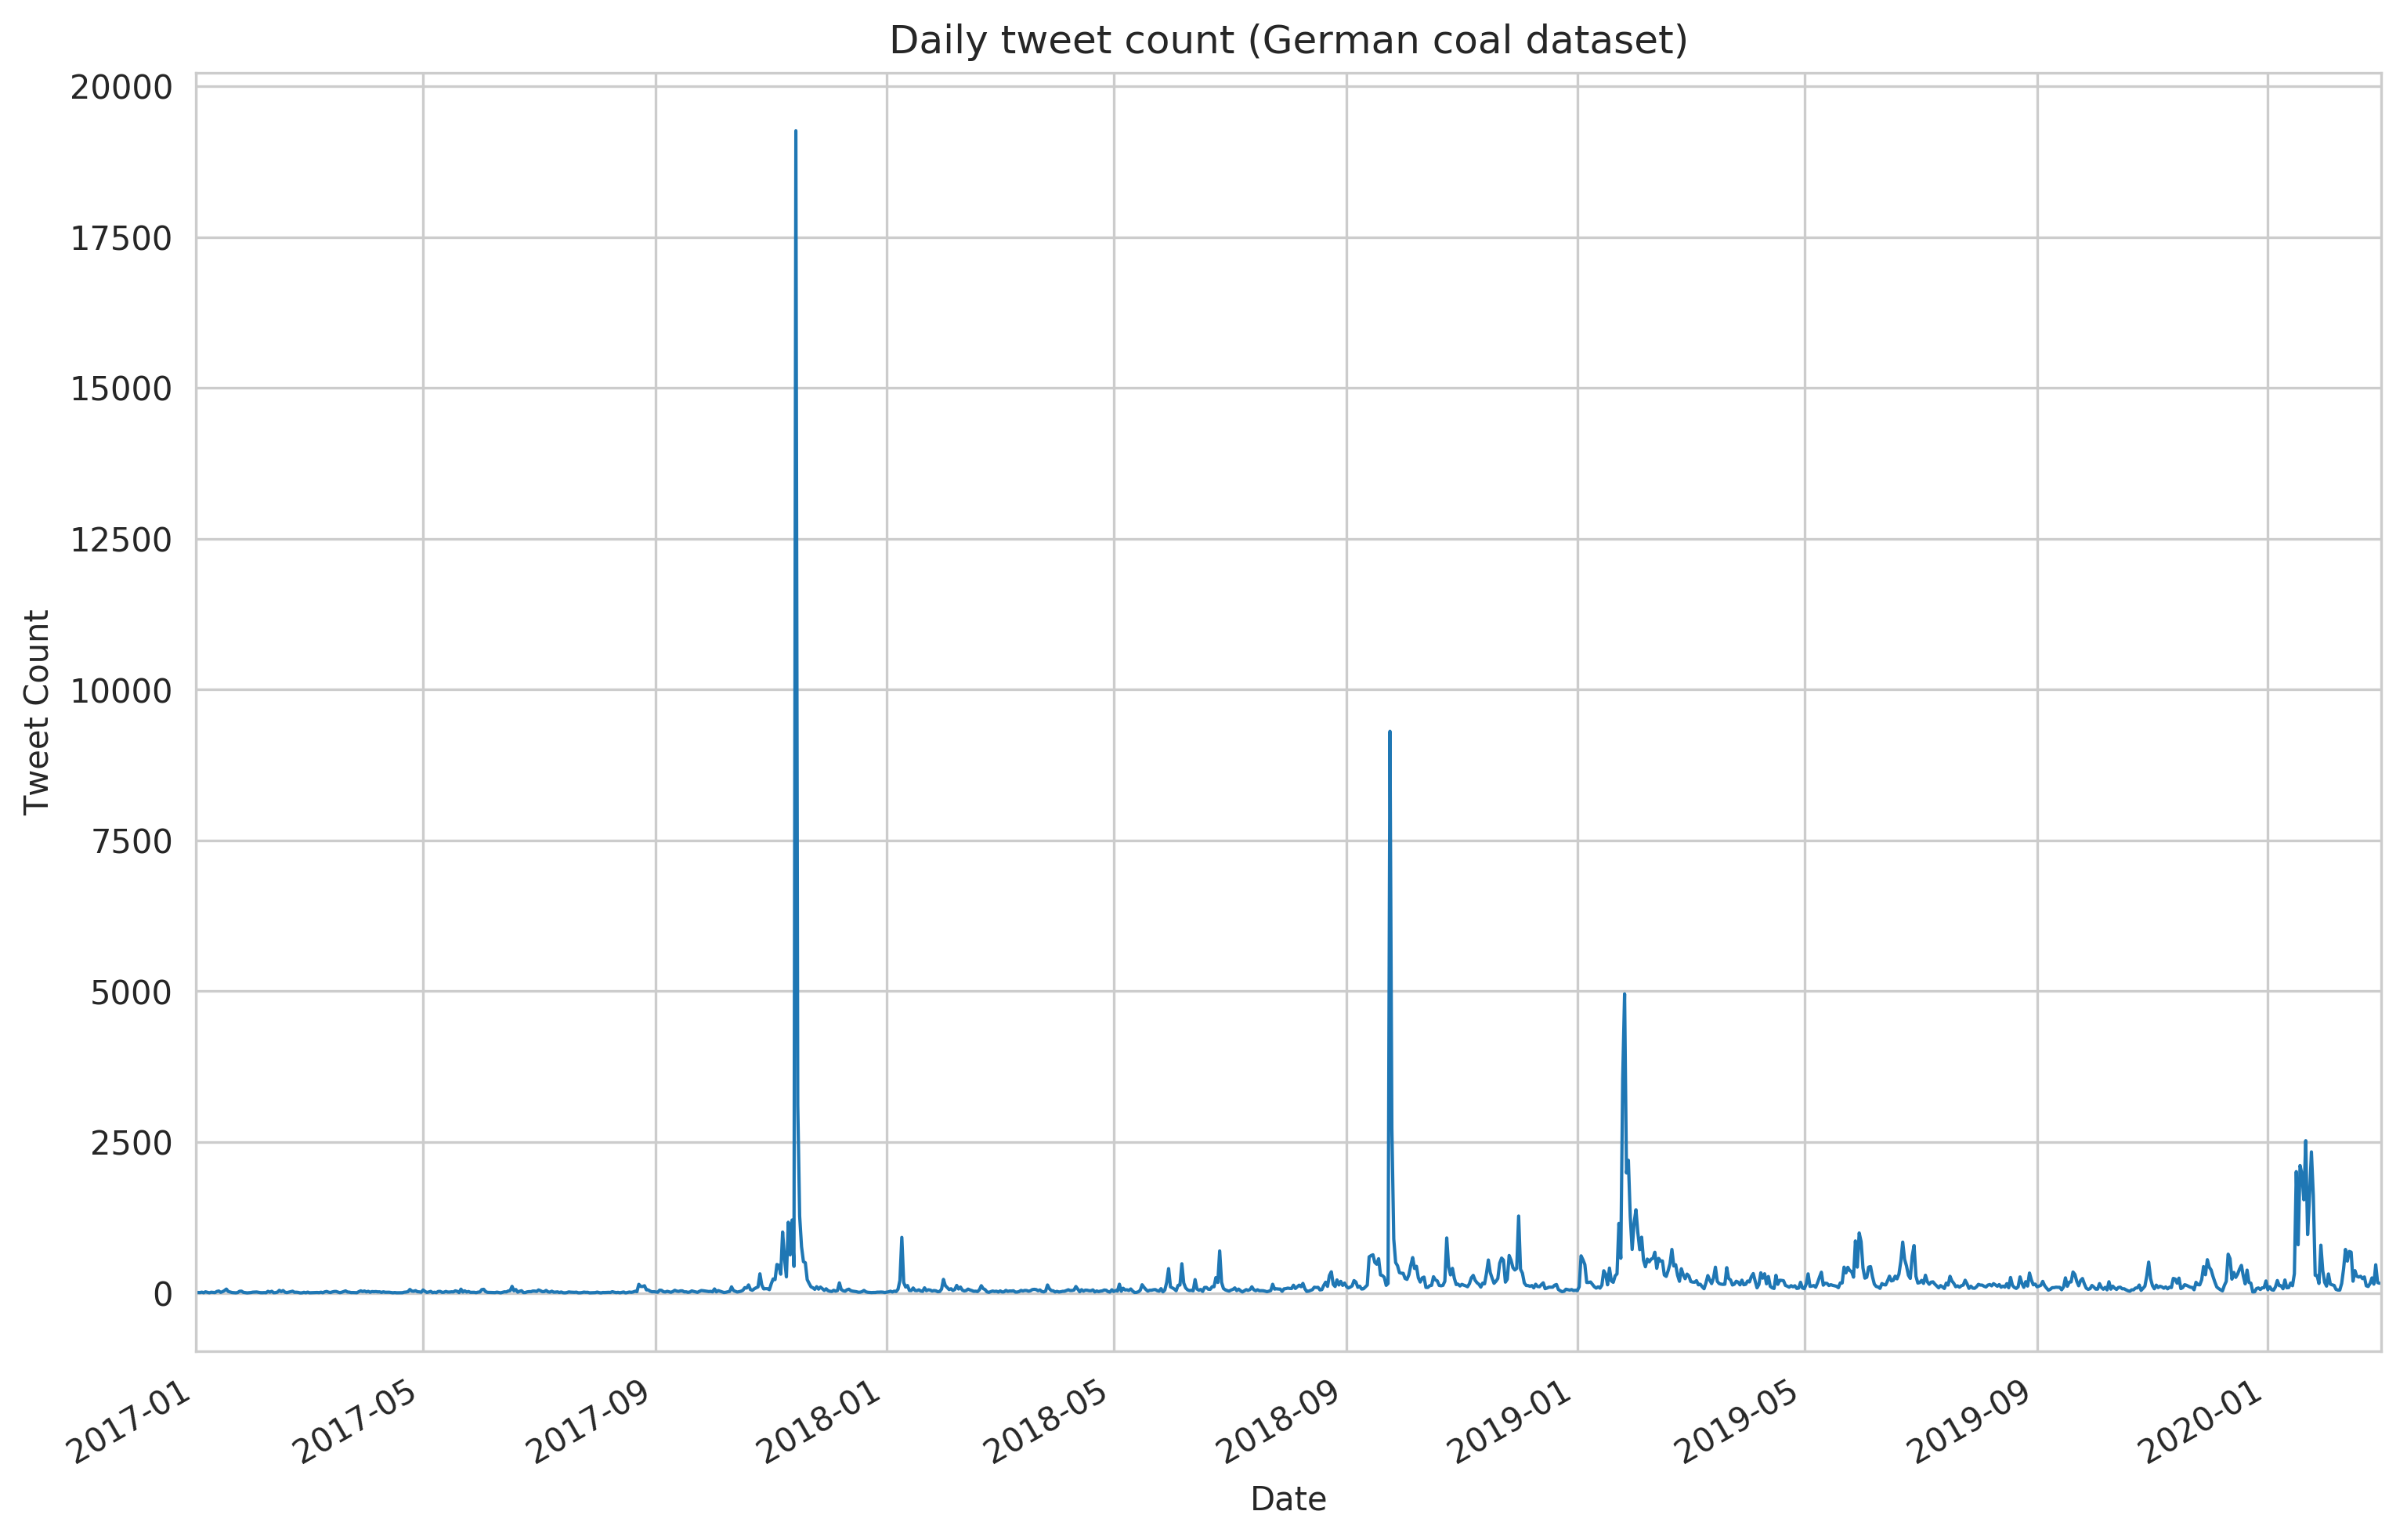
\includegraphics[width=0.9\linewidth]{figures/sa_tweet_frequency_zoom4}
	\end{center}
	\caption{\textbf{Daily frequency of German tweets in coal dataset over coal commission process.} The frequency remains quite stable over time, showing a slight increase over time, with periods of increased activity in December 2017, between September 2018 and February 2019, and in January 2020.}
	\label{fig:tweet_frequency}
\end{figure}

\section{Method} \label{sec:method}
% [T: 800, C: 750]
\subsection*{Sentiment Analysis.}
% Explanation of sentiment analysis

Sentiment analysis refers to the use of natural language processing and text analysis to systematically identify and extract affective states and subjective information in text. % cite?

The dictionary used is SentiWS, a publicly available German-language resource for sentiment analysis \citep{REMUS10.490}. Entries in the SentiWS dictionary set have four components: the word, its Part of Speech (POS) tag, a polarity weight, and inflections associated with the word, as seen in Fig. \ref{fig:sentiws_example}. The semantic orientations of the words are obtained from three different sources with manual revision.

The weights of word entries in SentiWS are retrieved using a method known as \emph{Pointwise Mutual Information} (PMI), first suggested in \citep{church-hanks-1990-word}. This approach was successfully re-used for sentiment analysis -- the determination of the semantic orientation and the strength of adjectives -- in \citep{Turney2002} and \citep{Turney2003}, where semantic orientation is inferred from \emph{semantic association}. The semantic orientation \(SO\) of a given word \(w\) is calculated from the strength of its association \(A\) with a manually-selected set of positive seed words \(P\) minus the strength of its association with a set of negative seed words \(N\) (cf. Equation \ref{eq:semantic_orientation}).

\begin{equation}
\label{eq:semantic_orientation}
\text{SO-A}(w) = \sum_{p \in P}A(w,p) - \sum_{n \in N}A(w,n)
\end{equation}

The word \(w\) is classified as having a positive semantic orientation when SO-A(\(w\)) is positive and a negative semantic orientation SO-A(\(w\)) is negative. The absolute value of SO-A(\(w\)) can be considered the strength of its semantic orientation.

Parallel to the paradigms in \citep{Turney2003}, SentiWS uses a set of German seed words, from which the semantic associations \(A(w,p)\) and \(A(w,n)\) are calculated using PMI (Equation \ref{eq:pmi}):

\begin{equation}
\label{eq:pmi}
\text{PMI}(w_1,w_2) = \log_2\left(\frac{P(w_1 \& w_2)}{P(w_1) \cdot P(w_2)}\right)
\end{equation}
where \(P(w)\) is the probability that \(w\) occurs and \(P(w_1 \& w_2)\) is the probability that \(w_1\) and \(w_2\) co-occur. The probabilities were estimated using frequencies and co-occurrence statistics on an internal German-language corpus by the creators of SentiWS consisting of approximately 100 million sentences. The final weights are then scaled to the interval of [-1;1] and rounded to 4 decimal places with +1.0 being absolutely positive and -1.0 being absolutely negative.

\begin{figure}
	\begin{center}
		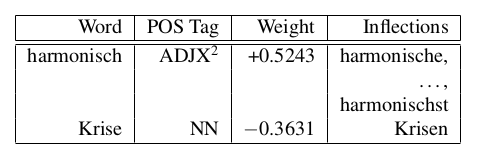
\includegraphics[width=0.5\linewidth]{figures/sentiws_example2}
	\end{center}
	\caption{Example of scoring a tweet using the polarity weighting of words from SentiWS. Source: \citep{REMUS10.490}}
	\label{fig:sentiws_example}
\end{figure}

To obtain the sentiment score of a tweet, denoted by \(s_{tweet}\), the following formula is used:

\begin{equation}
\label{eq:word_score}
s_{tweet} = \frac{\sum_{i=1}^{n} s_i f_i}{\sum_{i=1}^{n} f_i}
\end{equation}
where \(s_i\) is the polarity weighting score of a word given in SentiWS, and \(f_i\) is the frequency of occurrence of the word in the tweet.

\begin{figure}
	\begin{center}
		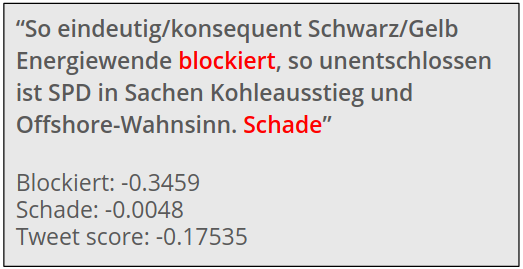
\includegraphics[width=0.5\linewidth]{figures/sentiws_example_use}
	\end{center}
	\caption{Schema of SentiWS entries}
	\label{fig:sentiws_example_use}
\end{figure}

Fig. \ref{fig:sentiws_example_use} shows an example of how the polarity weights from the SentiWS dictionary is used to score a tweet from the coal dataset\footnote{Translation: As unambiguously/consistently black/yellow as the energy turnaround is blocked, so indecisively is the SPD on the coal exit and offshore madness. A pity}. The words ``blockiert'' and ``schade''\footnote{Translation: Blocked, Pity} are the only two words that have non-zero polarity weighting scores in the dictionary, so the sum of the scores of the two words is taken and averaged over the number of scored words (2 in this tweet) to arrive at a average tweet sentiment score of -0.175.

\subsection*{Word Shift.}
% Explanation of word shifts
Building upon the analysis of tweet sentiment scores, word shift graphs represent a measure of the variation between the sentiment scores of two sets of texts. In these graphs, words are ranked by their descending absolute contribution to the change in average sentiment score between two sets of texts.

As tweets comprise words, the approach for finding the absolute contributions will be conducted on the word-level. If we consider two sets of texts, \(T_{ref}\) (reference) and \(T_{comp}\) (comparison) with average scores of \(s_{\text{avg}}^{\text{ref}}\) and \(s_{\text{avg}}^{\text{comp}}\) respectively, to compare both texts, we write:

\begin{equation}
\label{eq:text_difference}
T_{comp} - T_{ref} = \frac{\sum_{i}^{N} s_i f_i^{\text{comp}}}{\sum_{i=1}^{N} f_i^{\text{comp}}} - \frac{\sum_{i,ref}^{N} s_i f_i^{\text{ref}}}{\sum_{i=1}^{N} f_i^{\text{ref}}}
\end{equation}
where \(s_i\) is the polarity weighting score of a word given in SentiWS, and \(f_i\) is the frequency of occurrence of the word in the entire text set.

Equation \ref{eq:text_difference} shows the difference between the normalised score product of each word in the two text sets, and the absolute numbers are then ranked.

All data collection, pre-processing, and analysis was done using the programming language Python\footnote{All code for data pre-processing and analysis is available on the author's GitHub at: \href{https://github.com/yuantinglee/twitter-discourse}{https://github.com/yuantinglee/twitter-discourse}}.  

\section{Results} \label{sec:results}
% [T: 3.5K]

\begin{figure}
	\begin{center}
		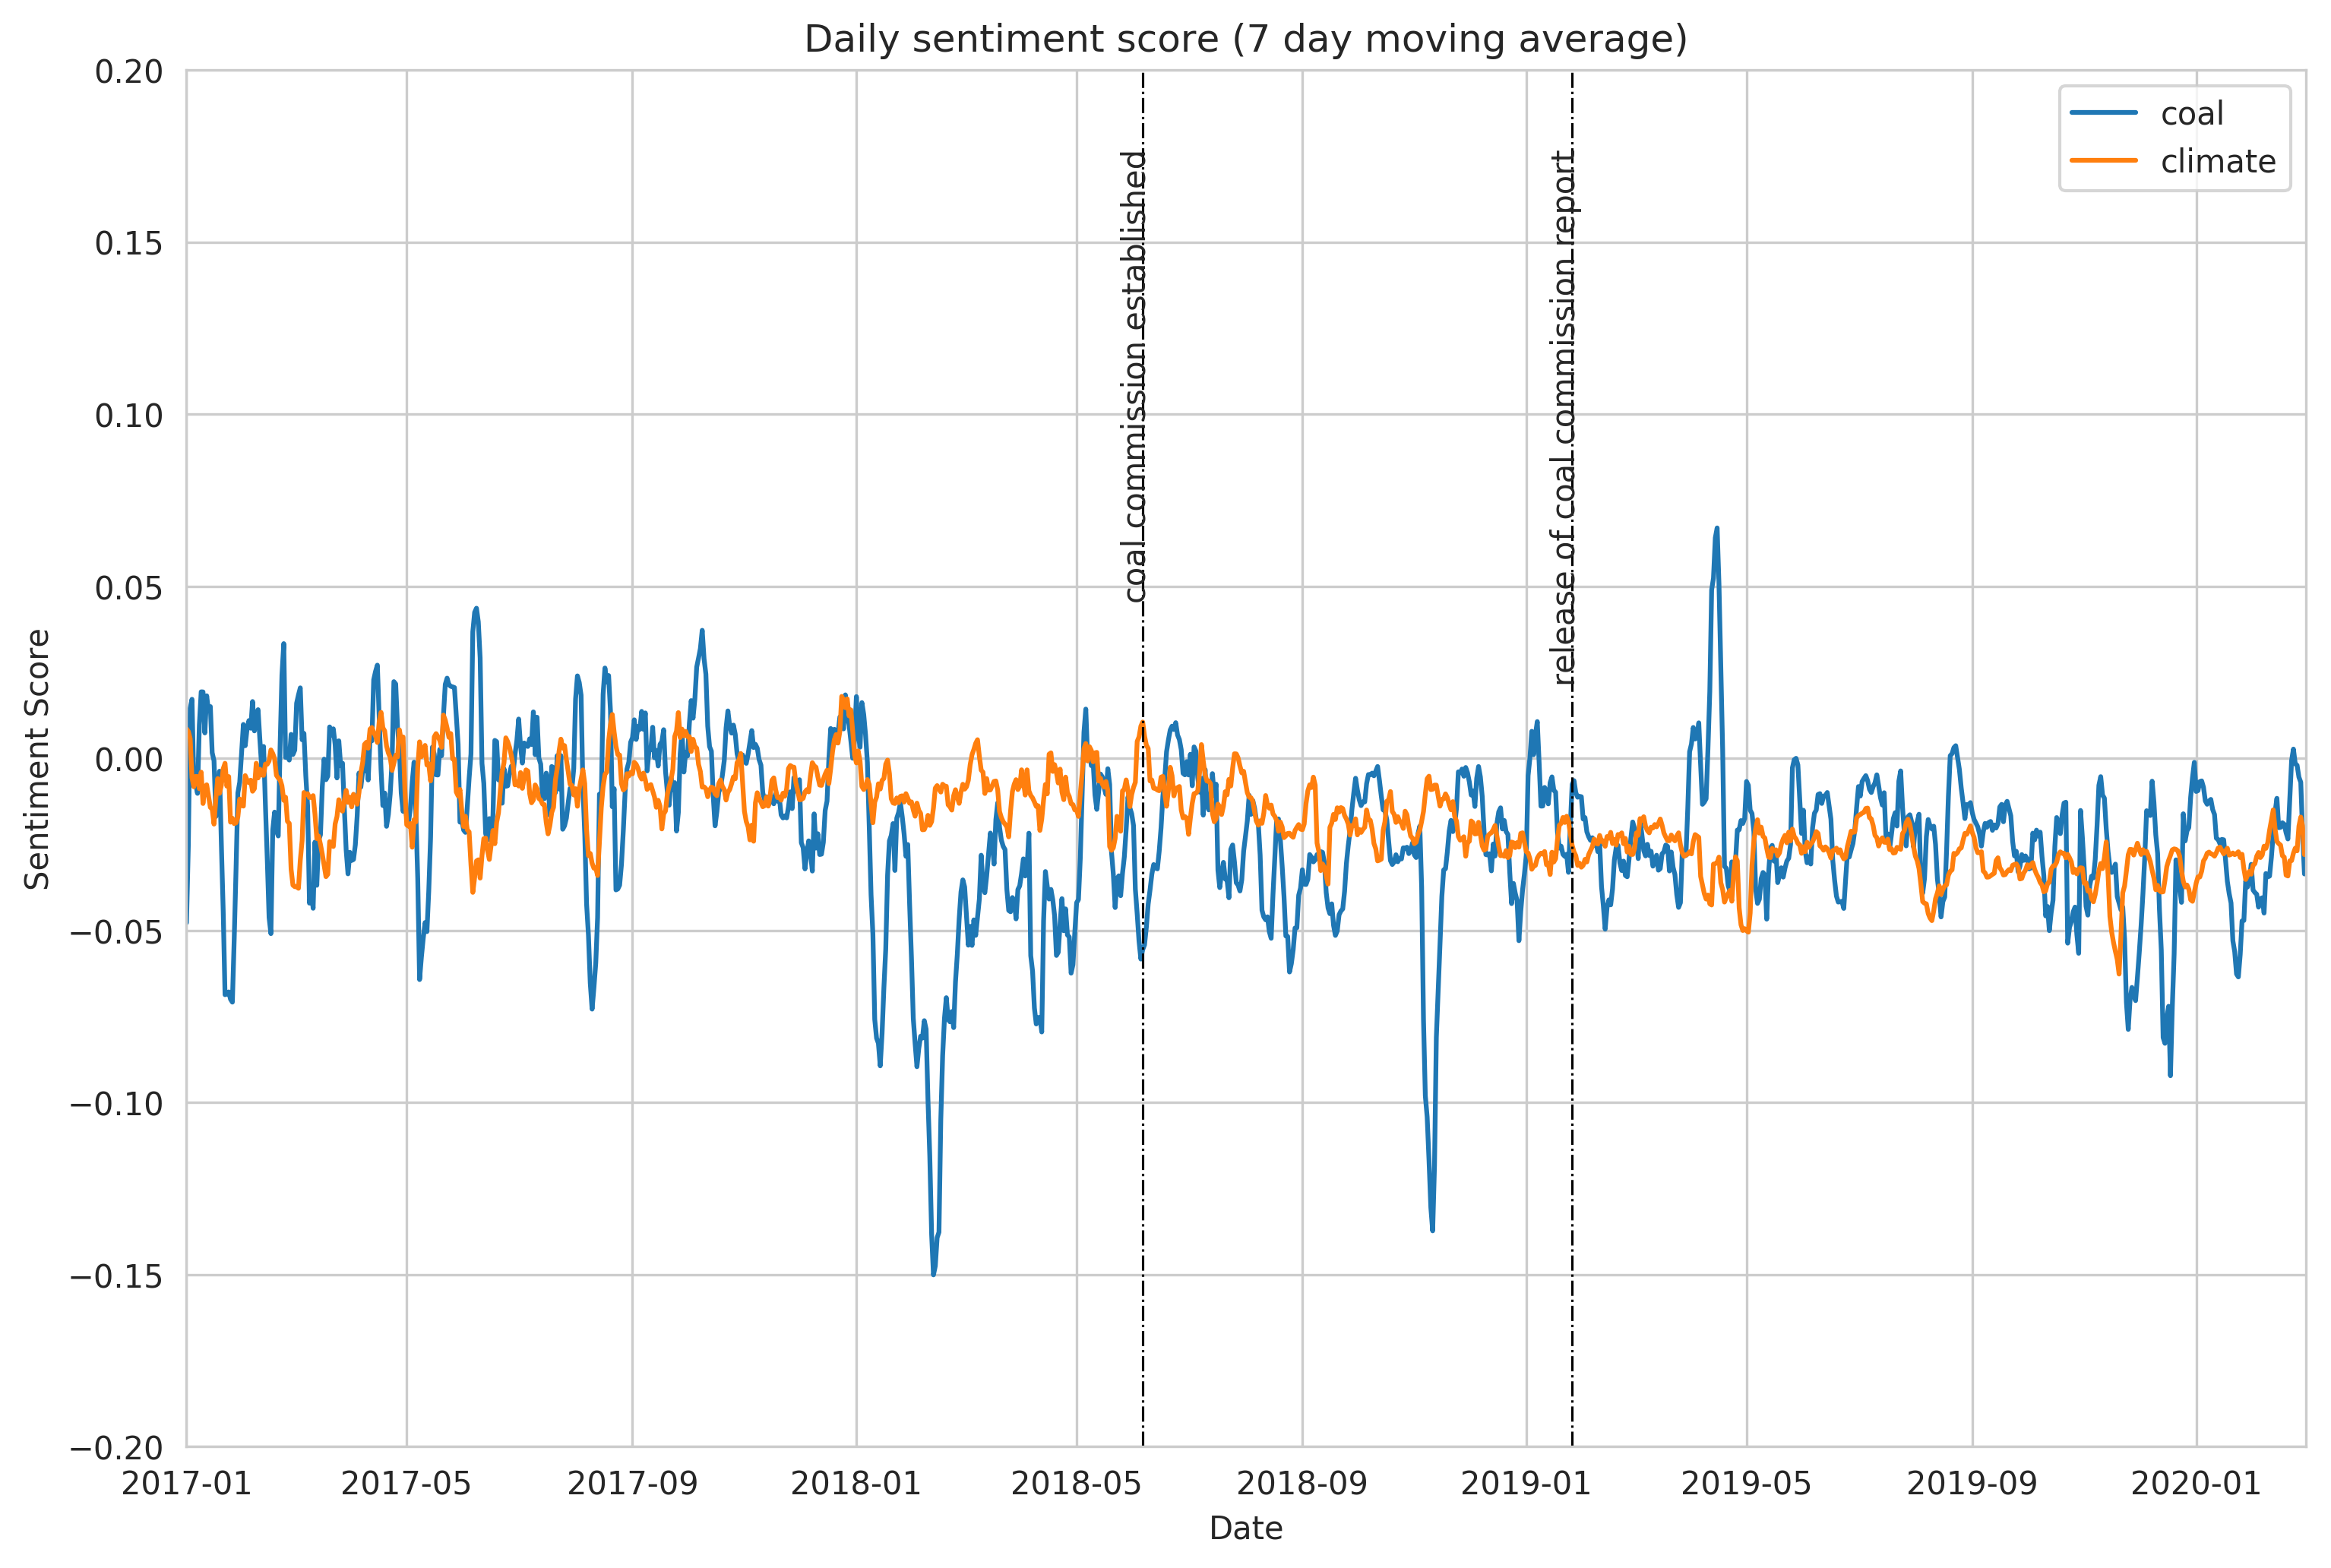
\includegraphics[width=\linewidth]{figures/sa_dailyavgsenti_7dma_baseline2}
	\end{center}
	\caption{\textbf{Sentiment score of tweets over time, expressed as a 7 day moving average.} Both scores show a negative trend over time, and there is greater variation in the average sentiment scores for coal tweets compared to climate.}
	\label{fig:tweet_score}
\end{figure}

\subsection*{Sentiment scores against time.}
% [T: 900, C: 750]
\subsubsection*{Negative trend} % overall trend negative
Fig. \ref{fig:tweet_score} shows the 7 day moving average of tweet scores in the coal and climate datasets. Looking at Fig. \ref{fig:tweet_score}, the first observation that can be drawn is that the average sentiment scores of both coal and climate tweets decrease over time. For most of 2017, the average score of coal and climate tweets hover around zero. This average for the climate tweets starts to decrease from the beginning of 2018, and steadily declines throughout the process of the coal commission, and remains constant around -0.025 even after the conclusion of the coal commission process. For the coal tweets, the average drops from the beginning of 2018 and remains constant around the -0.025 score as well.

Regression analysis also shows that the two time series have a negative slope. The slope of the coal timeseries is $-1.91 \times 10^{-5}$ and the slope of the climate timeseries is $-2.64 \times 10^{-5}$. In order to perform linear regression on dates, the dates are first converted into ordinal numbers. This suggests that the language used in both coal and climate discussions become more negative over time, of which the coal commission could have had an effect on.

\subsubsection*{Variation in coal and climate scores} % similar before and after but not during
Another observation that can be made is that the shape of the coal and climate timeseries correlate quite well both before and after the process of the coal commission, but not during. Looking at Fig. \ref{fig:tweet_score}, by breaking down the dates into three periods -- i. January 2017 to December 2017, ii. January 2018 to April 2019 and iii. May 2019 to February 2020, the differences in the sentiment score timeseries can be dissected. The spikes in the coal and climate tweet sentiment scores follow quite closely to each other in the first period, as well as in the third. However, they differ greatly in the second period, largely due to the variation of scores in the coal debate.
% add some numbers here to substantiate

% greater variation in coal compared to climate
In addition to the timeseries trends, comparing the two sentiment score timeseries of coal and climate tweets, it can be seen that there is a larger variation in sentiment scores in the coal dataset compared to that of climate. This is evident across the entire time period of the dataset. Throughout 2017, the variation in climate scores is 0.057, compared to 0.116 in the scores of coal tweets. This difference increases in the period surrounding as well as during the coal commission process from January 2018 to April 2019, where the variation in climate tweet scores is 0.061, compared to 0.217 in the scores of coal tweets. The difference in variation of the tweet scores between the datasets declines after the coal commission process, with a variation of 0.048 in climate tweets and 0.096 in coal tweets from May 2019 to February 2020.

% table on absolute variation
% {\color{red}FIX NAN VALUES}
\begin{table}[htbp]
	\begin{center}
		\caption{Variation in daily average  and 7 day moving average sentiment scores of coal and climate tweets}
		\label{table:score_variation}
		\begin{tabular}{| l | l| l | l | l | l| l | l | l | l| l | l | l |}
			\hline
			\multicolumn{13}{ |c| }{Sentiment scores} \\ \hline
			& \multicolumn{6}{ |c| }{Daily average} & \multicolumn{6}{ |c| }{7 day moving average} \\ \hline
			& \multicolumn{3}{ |c| }{Coal} & \multicolumn{3}{ |c| }{Climate} & \multicolumn{3}{ |c| }{Coal} & \multicolumn{3}{ |c| }{Climate} \\ \hline
			Period & I & II & III & I & II & III & I & II & III & I & II & III \\ \hline
			Maximum score & 0.189 & 0.207 & 0.067 & 0.054 & 0.058 & -0.001 & 0.044 & 0.067 & 0.004 & 0.018 & 0.011 & -0-014 \\ \hline
			Minimum score & -0.191 & -0.297 & -0.293 & -0.108 & -0.130 & -0.118 & -0.073 & -0.150 & -0.092 & -0.039 & -0.050 & -0.063 \\ \hline
			Difference & 0.379 & 0.504 & 0.360 & 0.162 & 0.189 & 0.118 & 0.116 & 0.217 & 0.096 & 0.057 & 0.061 & 0.048 \\ \hline
		\end{tabular}
	\end{center}
\end{table}

Here, consensus could be measured using a proxy, through the variation in positive and negative tweet scores, where a large difference denotes less consensus and a smaller difference denotes a greater consensus. The sentiment score timeseries thus suggests that consensus in the coal debate decreased across the period surrounding the coal commission, compared to before and after. In contrast, the consensus in the climate debate remains relatively stable over time.

% greater variation around CC period;
Looking at the coal debate during the period starting slightly before the establishment of the commission (January 2018) to slightly after the findings of the coal commission was published (May 2019), the absolute variation in tweet scores during this period is much larger compared to the periods before and after. As suggested previously, this could be linked to public consensus in the debate and suggest that the process of the coal commission led to both an increase in the coal debate on Twitter (as shown from the tweet frequencies in Fig. \ref{fig:tweet_count_event_timeline}) and less public consensus on Twitter as a result of an increase in debate.

% Summary
Overall, analysis of the sentiment scores of the coal and climate debate on Twitter reveals that there are some similarities, in that they both become more negative over time and have similar trends, but largely differ from each other during the period surrounding the coal commission process. In order to understand why they differ, however, it is necessary to look into the tweets that drive the differences between the coal debate and the climate debate. Doing so will allow better understanding of the events that drive these differences and whether the coal commission process is linked to it.

\begin{figure*}
	\begin{center}
		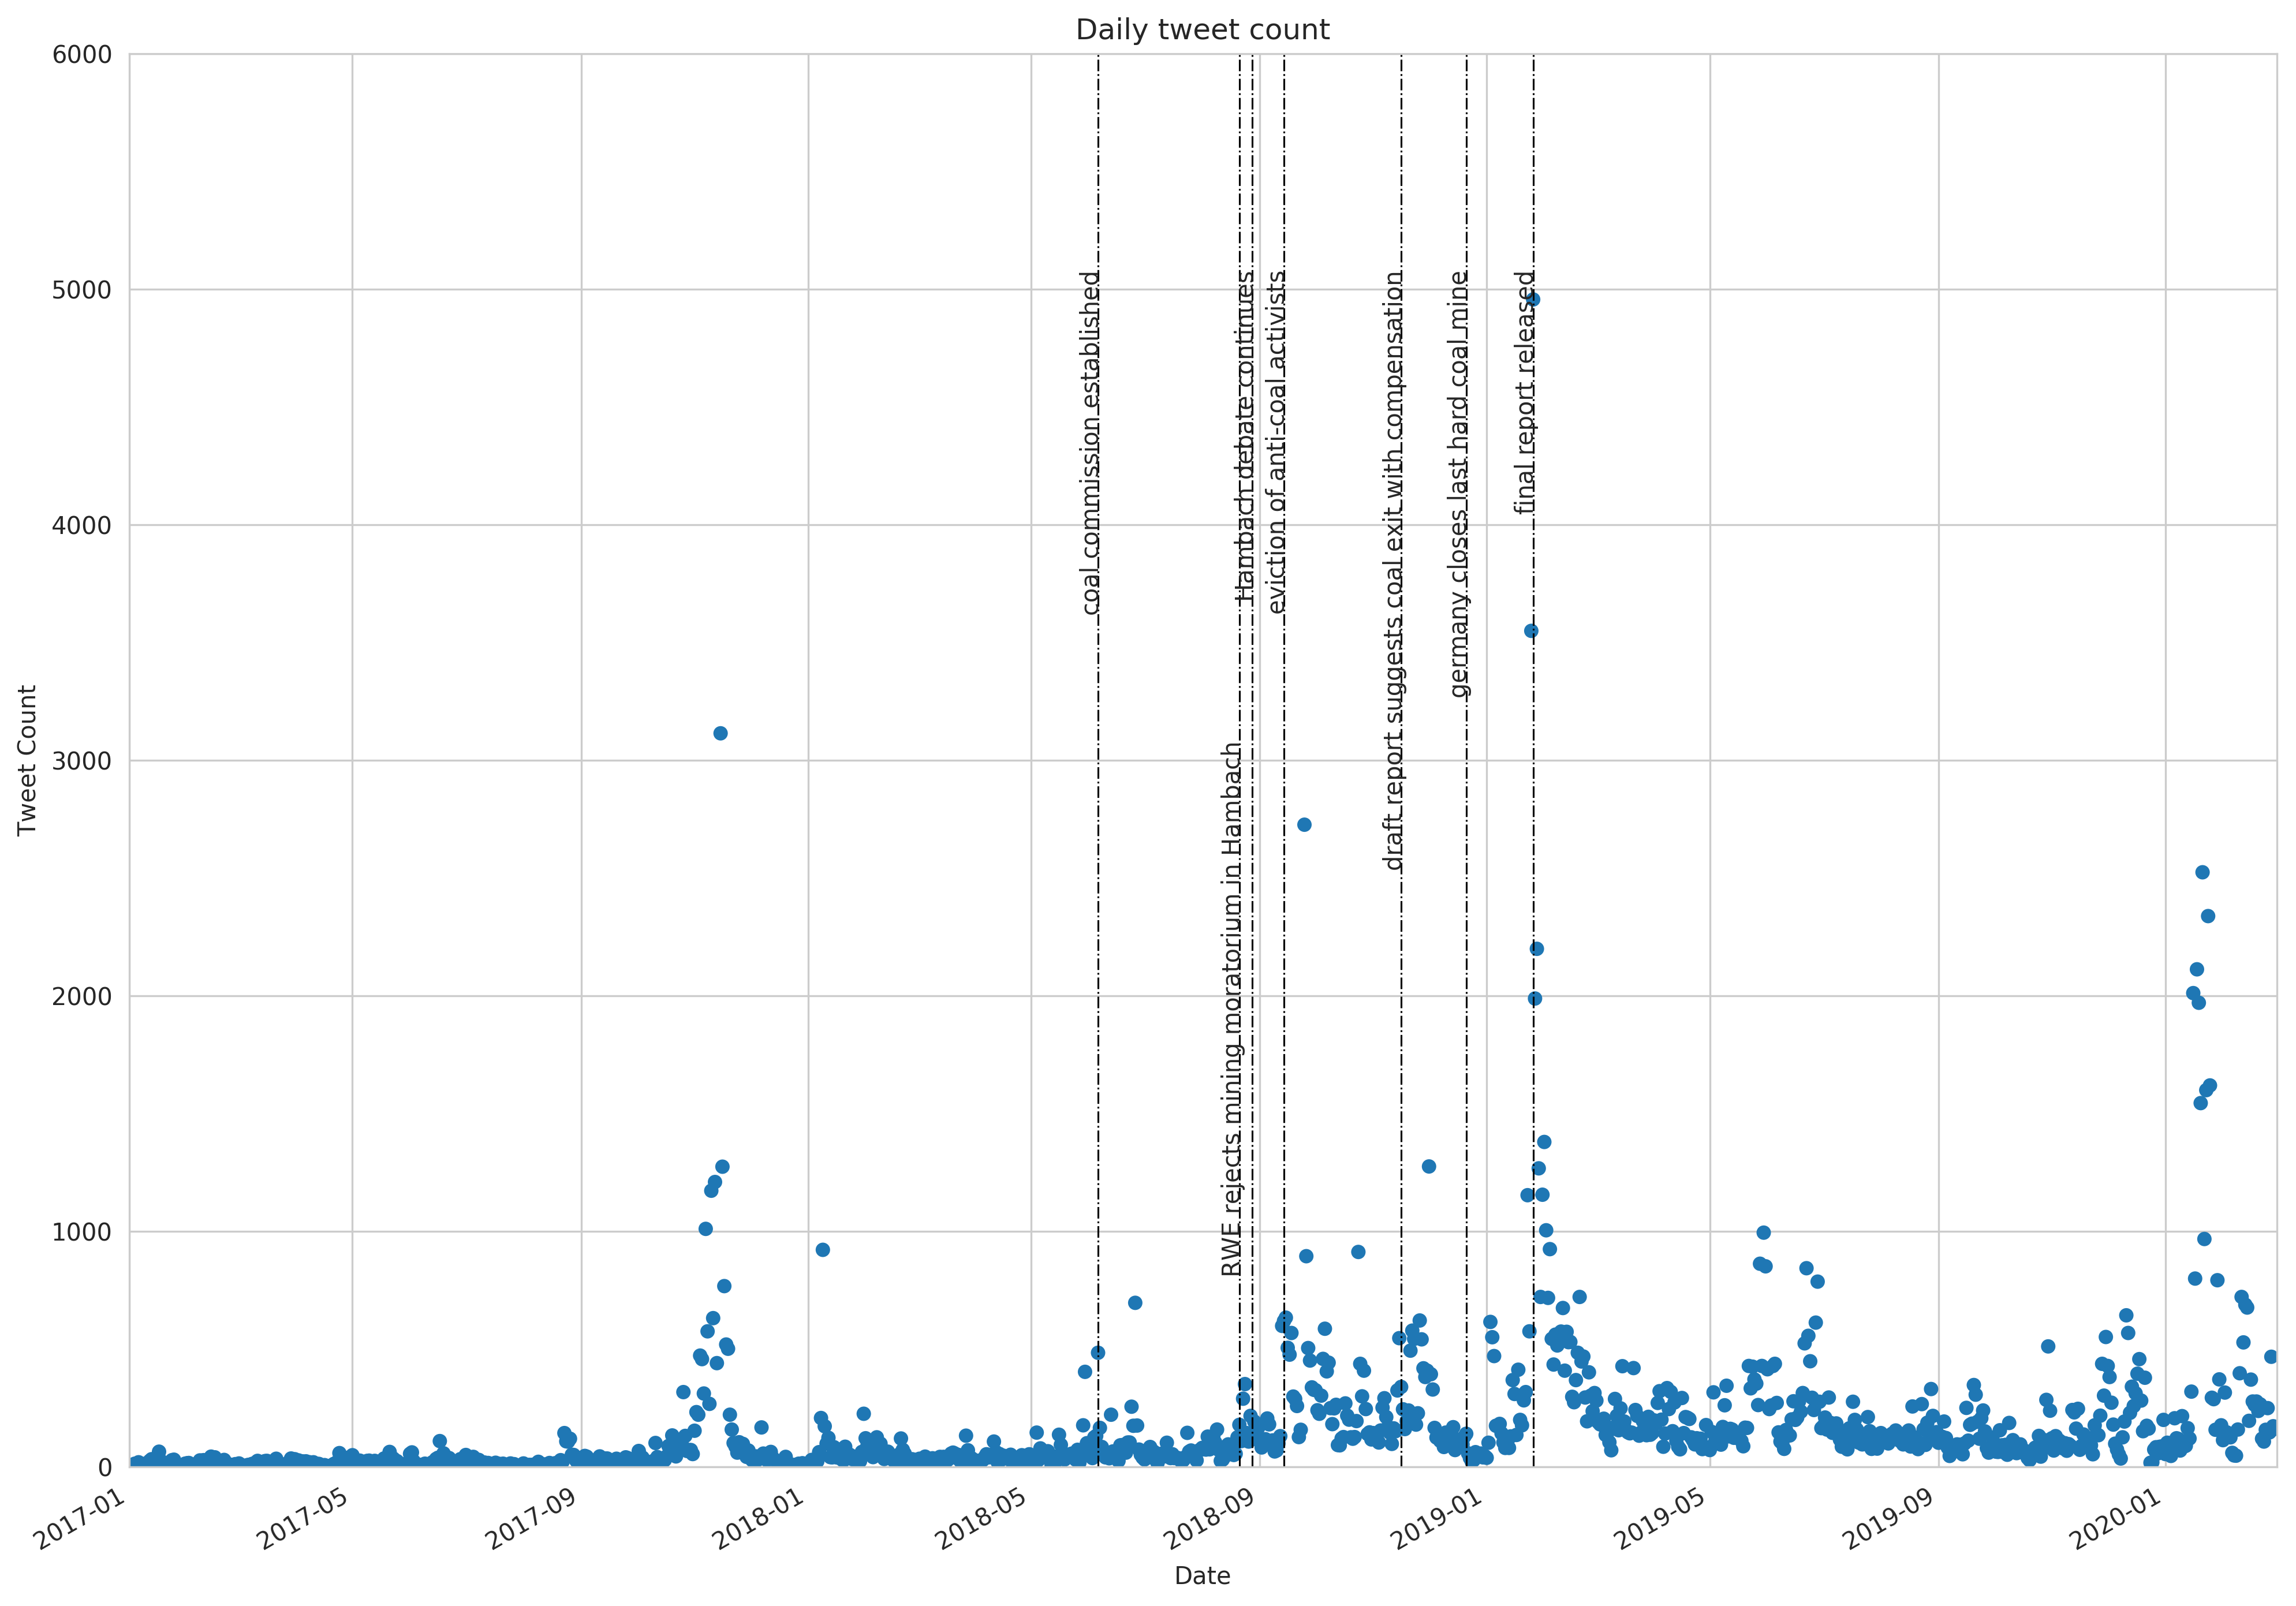
\includegraphics[width=\textwidth]{figures/sa_tweet_count_event_timeline3}
	\end{center}
	\caption{\textbf{Daily count of tweets throughout coal commission process against events throughout coal commission process.} There appears to be an uptick in the frequency of tweets during the period of the coal commission, especially during the occurrence of important events.}
	\label{fig:tweet_count_event_timeline}
\end{figure*}


\subsection*{Event Analysis.}
% [T: 1600, C: 1580]
Fig. \ref{fig:tweet_count_event_timeline} shows the daily count of tweets throughout the coal commission process against events throughout the same process. In Fig. \ref{fig:tweet_count_event_timeline} and \ref{fig:tweet_score_event_timeline}, the date of significant events are overlaid on the same plot as the daily average sentiment score of tweets. Significant events from the coal commission process were taken from Clean Energy Wire's report on the events following the coal commission \citep{Amelang2019}.

\begin{figure*}
	\begin{center}
		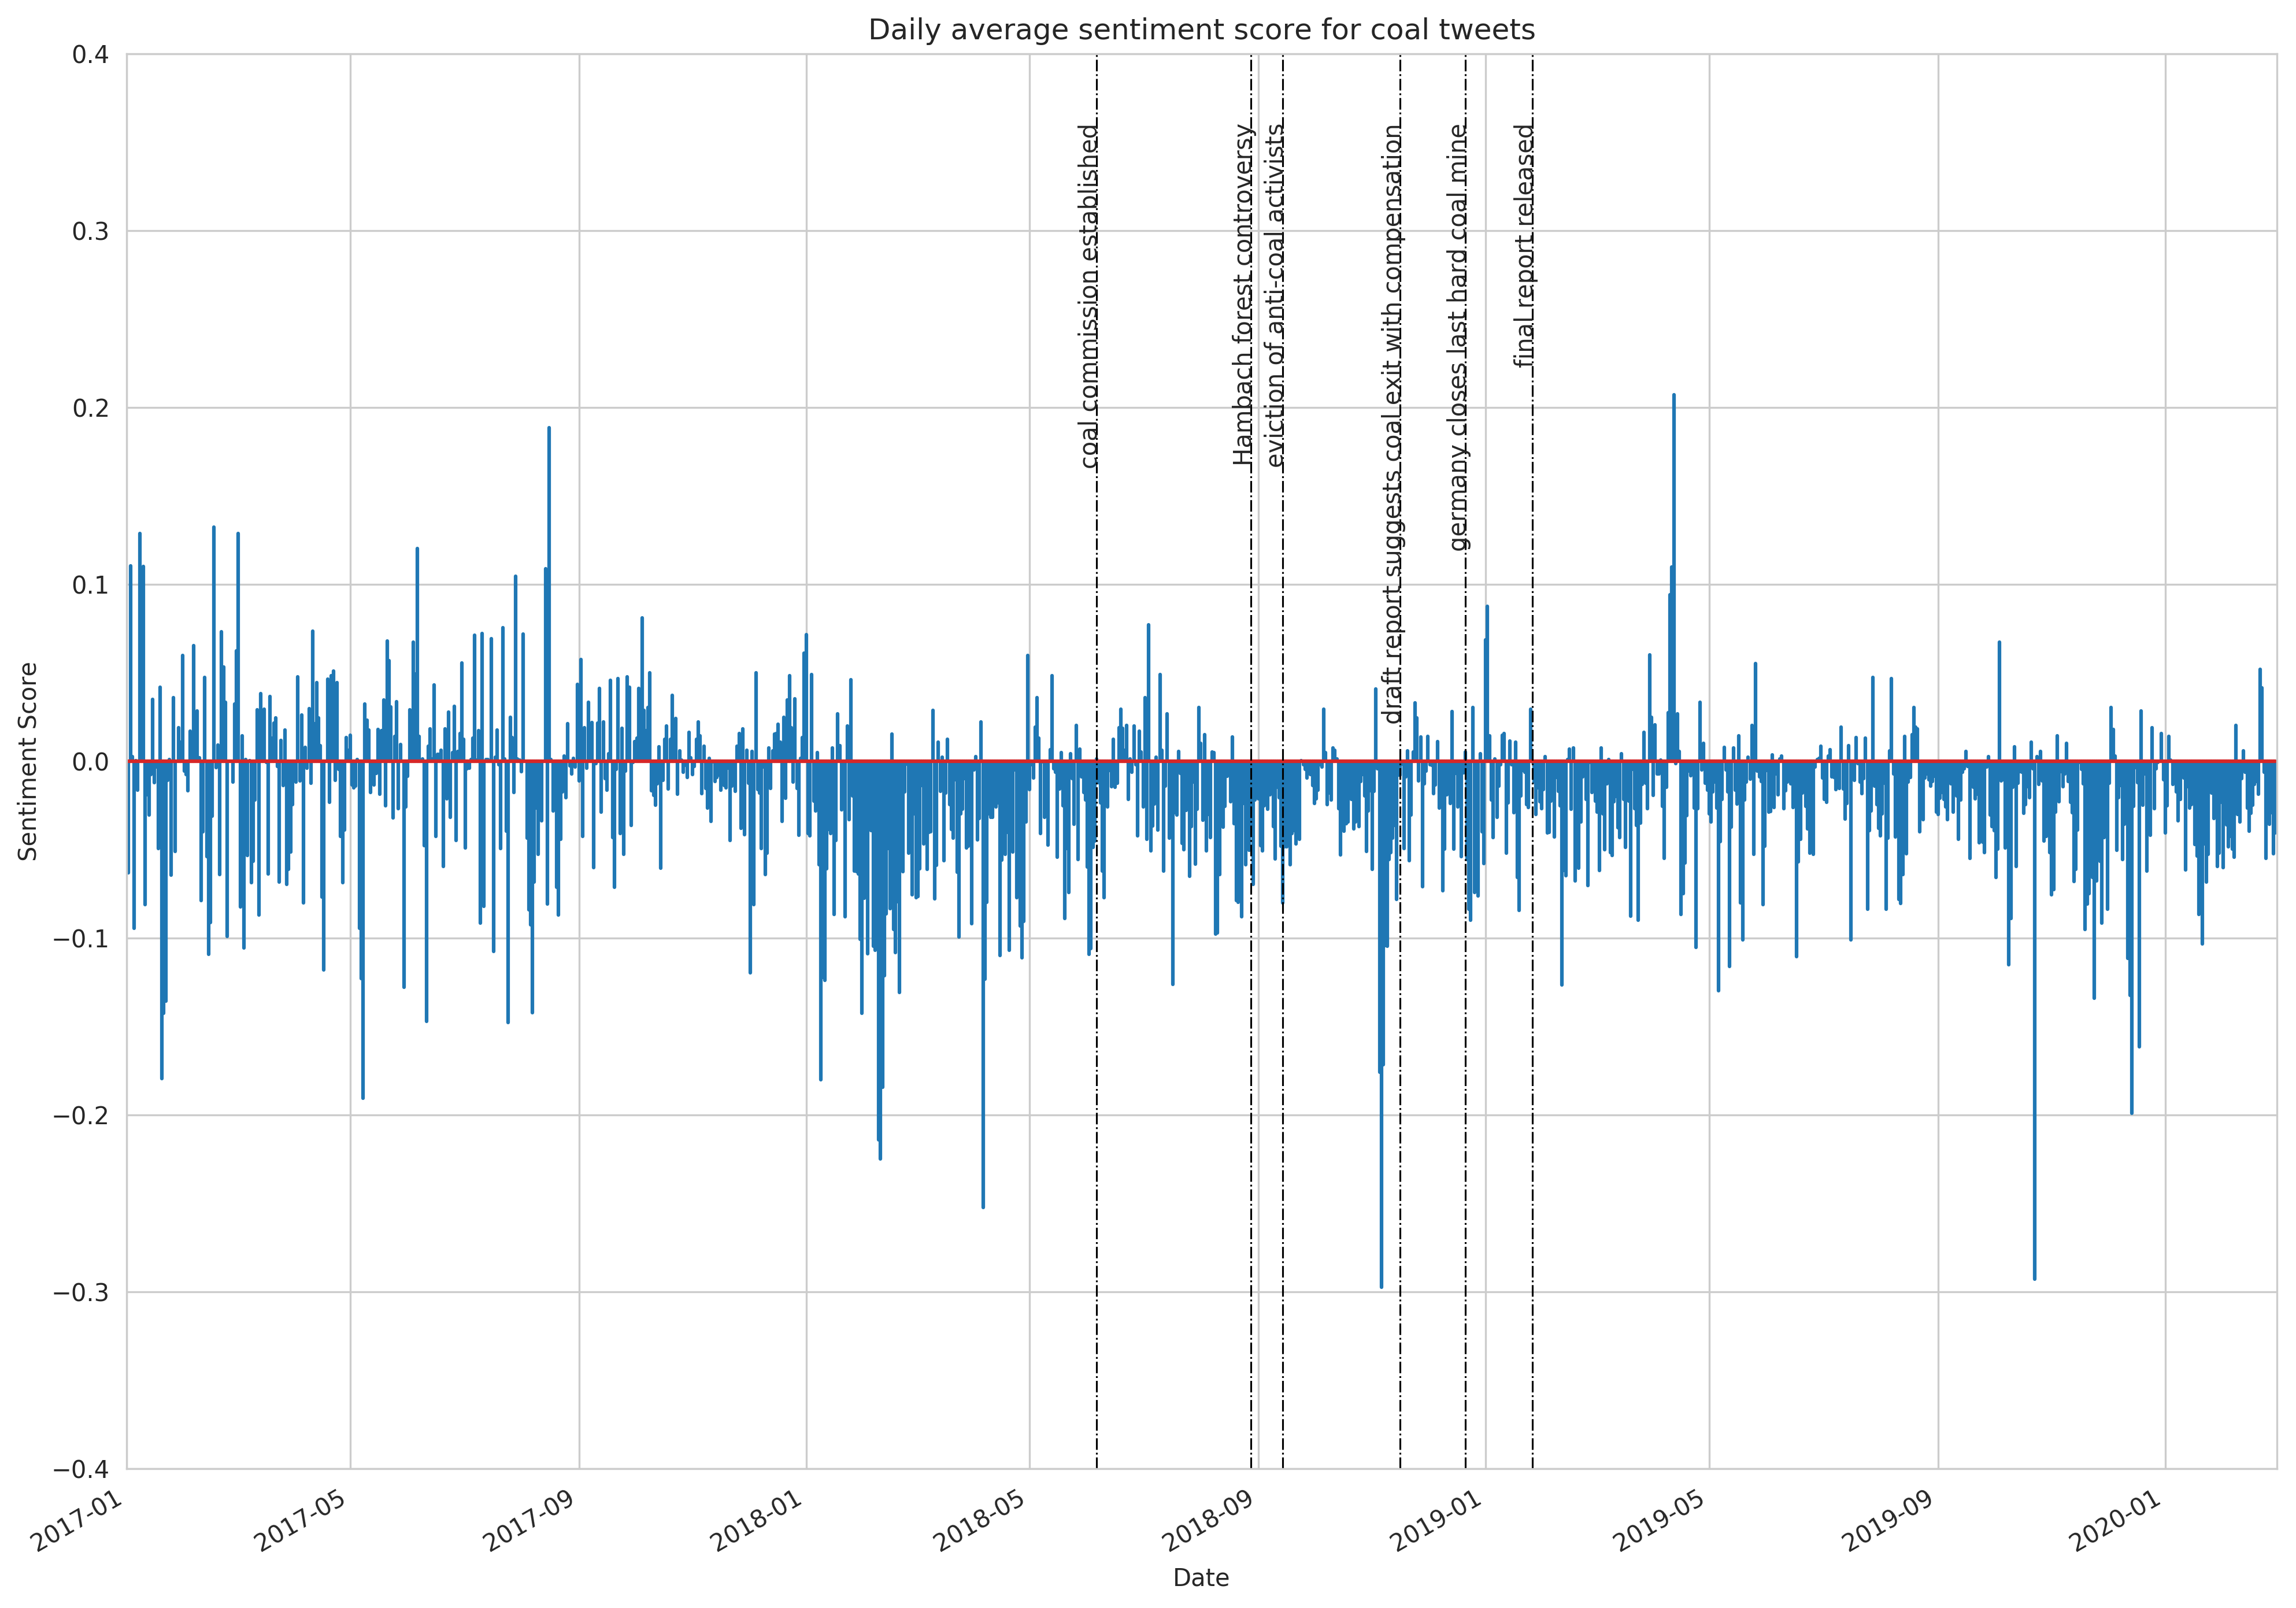
\includegraphics[width=\textwidth]{figures/sa_tweet_score_event_timeline3}
	\end{center}
	\caption{\textbf{Daily average sentiment score of tweets against events throughout coal commission process.} In contrast to tweet frequency, there does not appear to be a strong correlation between the occurrence of important events throughout the process of the coal commission and the daily average sentiment score.}
	\label{fig:tweet_score_event_timeline}
\end{figure*}

A further look at specific events in Fig. \ref{fig:tweet_count_event_timeline} show that there is an uptick in the frequency of tweets when significant events take place. In particular, the day with the most number of tweets in the dataset was on the 26 January 2019, which was when the coal commission released its final report with recommendations on how to manage the coal phase-out in Germany. The average number of tweets made per day is also higher in the period surrounding the coal commission process at 223 per day compared to before 114. However, there is an increase in the average daily tweets made over time, as 245 tweets are posted per day on average in the period after the coal commission process. Here, the dates that are used for the three periods follow the same three that were defined in the previous section.

Looking at Fig. \ref{fig:tweet_score_event_timeline}, however, the variation in sentiment scores across time show that the tweets are not necessarily more extreme on the sentiment scale across the entire coal commission period. Rather, there are specific spikes in the scores slightly before the establishment of the coal commission, during the process of the coal commission, as well as after the conclusion of the coal commission with the release of its report.

\subsubsection*{Positive Peaks}
In Fig. \ref{fig:tweet_score_event_timeline}, there is only one large positive peak, on 11 April 2019. Analysis of the coal debate reveal that there was one specific tweet with a high sentiment score of 0.358 with 1100 retweets that was driving the high average tweet score for that day.

\begin{displayquote}
	\textbf{@Luisamneubauer}: Was die Regierung damit sagen möchte: Da hat die Kohlekommission ein Datum auf den Tisch gelegt, was uns so gut in den Kram passt - wäre ja schön blöd nur wegen so ein paar Halbstarken auf einmal echten Klimaschutz durchzusetzen, der wohlmöglich noch dem Parisabkommen entspricht.\footnote{Translation: What the government wants to say with this is that the coal commission has put a date on the table that suits us so well - it would be nice and stupid to suddenly push through real climate protection just because of a couple of youngsters, which would probably still be in line with the Paris Agreement.}
\end{displayquote}

In addition, there was another tweet posted on 9 April 2019, that also had a high sentiment score of 0.461 and generated a significant number of retweets (95).

\begin{displayquote}
	\textbf{@julia\_verbinden}: Großartig! \#DieAnstalt im @ZDF mit ``\#Scheuermann'' auf der Titanic, die ca 6 Grad Celsius vom Kurs nach \#Paris abgekommen ist. Mit ner \#Kohlekommission, die einen sowieso-\#Kohleausstieg vorschlägt, mit absurden Obergrenzen für \#Solarenergie uvm. \#Klimakrise \#FridaysForFuture\footnote{Translation: That is great! The institution on @ZDF with ``Scheuermann'' on the Titanic, which is about 6 degrees Celsius off course to Paris. With a coal commission, which proposes a coal exit anyway, with absurd upper limits for solar energy and much more.  \#Climate crisis \#FridaysForFuture}
\end{displayquote}

Looking at the two tweets in mention, the first observation that can be made is that they are both made by high-profile figures in Germany, which explains the high traction gained by the tweets. In the first example, Luisa Neubauer, the author of the tweet, is a German climate activist and one of the main organisers of the Fridays For Future movement in Germany, a school strike to protest the global climate situation \citep{FF20, FF20G}. In the second example, Dr. Julia Verbinden is a member of the German parliament, representing the Green Party \citep{Bundestag2020}. Both of the authors are supporters of strong climate action, and it is clear from the content of the tweets that they are not using positive words to express support for the coal commission. In the first example, the two highest scoring words -- ``gut'' and ``schön''\footnote{Translation: Good, Nice} are used in an ironic tone to criticise the German government for supporting what is perceived to be inadequate climate action proposed by the coal commission. In the second example, the word ``Großartig''\footnote{Translations: Great} is used to express support for a satirical show on German television that presented about the findings of the coal commission.

In both cases, the drivers for the spike in average tweet scores are not specific events, but rather due to Twitter posts by relatively high-profile figures on the network within the coal debate that criticise the coal commission or an element of the coal commission's report.

\subsubsection*{Negative Peaks} % negative peaks
Compared to positive peaks, there is a much larger amount of negative peaks seen in Fig. \ref{fig:tweet_score_event_timeline}. Of those, there is one large peak during the period which the coal commission was in session, on 6 November 2018. Further analysis reveal a single tweet that acted as the driver for the large negative spike, with an individual tweet score of -0.663, which had 201 retweets.

\begin{displayquote}
	\textbf{@ARTE:Re}: Kohle oder Wald, Arbeitsplätze oder Umwelt – am Streit um den \#HambacherForst Forst offenbart sich, dass das Thema Klimaschutz immer emotionaler wird. http://bit.ly/2AAXTvX \#hambi \#HambiGehtWeiter
	\footnote{Translation: Coal or forest, jobs or the environment - the dispute over the \#Hambach Forest reveals that the issue of climate protection is becoming increasingly emotional. http://bit.ly/2AAXTvX \#Hambi \#Go on Hambi}
\end{displayquote}

On Twitter, in addition to the text shown above, the post contains an embedded video which documents the protests by climate activists in the Hambach Forest in the state of North-Rhine Westphalia in Germany. The issue surrounding the Hambach forest was a point of contention during the process of the coal commission. In August 2018, the German energy company RWE rejected calls for a moratorium on the clearing of the forest as part of lignite mining, and said that it would continue mining operations there \citep{Knuf2018}. This was heavily criticised by environmental groups \citep{Schafer2018}, as well as by several member groups of the coal commission, some of which who threatened to leave the commission if RWE did not halt its mine expansion activities in the region while the coal commission was still in progress \citep{Wehrmann2018a}. The situation continued to escalate into September, as anti-coal activists began to occupy the forest and police action was taken to clear the activist camp \citep{CEW2018}. The debate continued, with RWE saying that not clearing the forest would cost billions of euros and that the forest could not be saved \citep{CEW2018a}, with environmental NGOs saying otherwise \citep{Kopiske2018}.

The tweet about the Hambach forest, thus, represents the view of the entire debate around the clearing of the Hambach forest with respect to the coal exit from environmentalists' perspective. This is reflected by the use of words with negative sentiments, contributing to a tweet that is critical about the coal exit.

In contrast, when looking at a negative peak before the coal commission process, which is that on 6 April 2018, the biggest driver of the negative spike on that day belonged to tweets with the same text content, amounting to a score of -0.367. What is interesting about this spike is that it is not a result of retweets of a tweet from an influential figure, but rather many different users posting the same text, presumably obtained from a website.

\begin{displayquote}
	\textbf{@reis\_theresa}: \#Kohlekraft macht krank. Die gefährlichen Abgase aus den Kohleschloten heizen unser Klima an – und sie schaden unserer Gesundheit. \#Weltgesundheitstag \#kohlefrei https://wwf.de/kohlefrei/kohl... via @WWF\_Deutschland
	\footnote{Translation: \#Coal power makes you sick. The dangerous exhaust gases from the coal chimneys heat up our climate - and they damage our health. \#World Health Day \#coal free https://wwf.de/kohlefrei/kohl... via @WWF\_Deutschland}
\end{displayquote}

Looking at the content of the tweet, the message is clear -- coal is postured as something that is bad for the environment, and negative language is used accordingly to represent that negative sentiment. The link provided in the tweet links to a page of World Wildlife Fund Germany, which reports on the results a survey that they commissioned about coal power in Germany, on the occasion of World Health Day on April 7th. The page also includes an option for readers to share the results of the survey on social media, including Twitter, and further asks for readers to sign a petition to demand for a coal exit.

The two cases highlight the different ways of communication on Twitter. One, as in the case of the tweet about the Hambach forest, is through retweets, which propagates across many different groups of people on Twitter as each user's retweet will appear on their followers' timeline. Another, as in the case of the tweet originating from the website of WWF Germany, shows how Twitter is used as a medium for other people to share information from other sources on the Internet.

In both cases, however, the negative sentiment arises from the usage of negative language to express the severity of the impacts that coal has on the environment. In the first example, it is negative sentiment comes from how a lack of a coal exit will result in further forest clearings, impacting biodiversity negatively and leading to more carbon emissions. In the second, the negative sentiment comes from criticising the environmental and health ill-effects of coal.

\subsection*{Word Shift.}
% [T: 850, C: 888]
In order to understand how the debate evolved over time, the tweet dataset used so far is split into two categories by date -- before the release of the report of the coal commission and after. The tweets that were made after the coal commission released its final report are then analysed in comparison to the tweets that were made before the report's release. This presents an opportunity to look at how the debate changed over time, whether the focus of the debate had changed after the coal commission began its decision-making process, and how public sentiment changed over the course of the same process.

To look at how the language and sentiment changed over time, a method known as ``word valence shift graphs'', first used in \citep{Dodds2011}, is employed. To do so, words are ranked by their absolute contributions to the change in average sentiment of one group relative to another. As detailed in the methods section, the top words driving the differences in the texts between the two periods are identified by finding the absolute differences in the product of the word frequency and word polarity in the two periods. The results are then plotted in Fig. \ref{fig:wordshift_coalcomm_report}.

% plus a zoom in on the sentiment score in that period
\begin{figure*}
	\begin{center}
		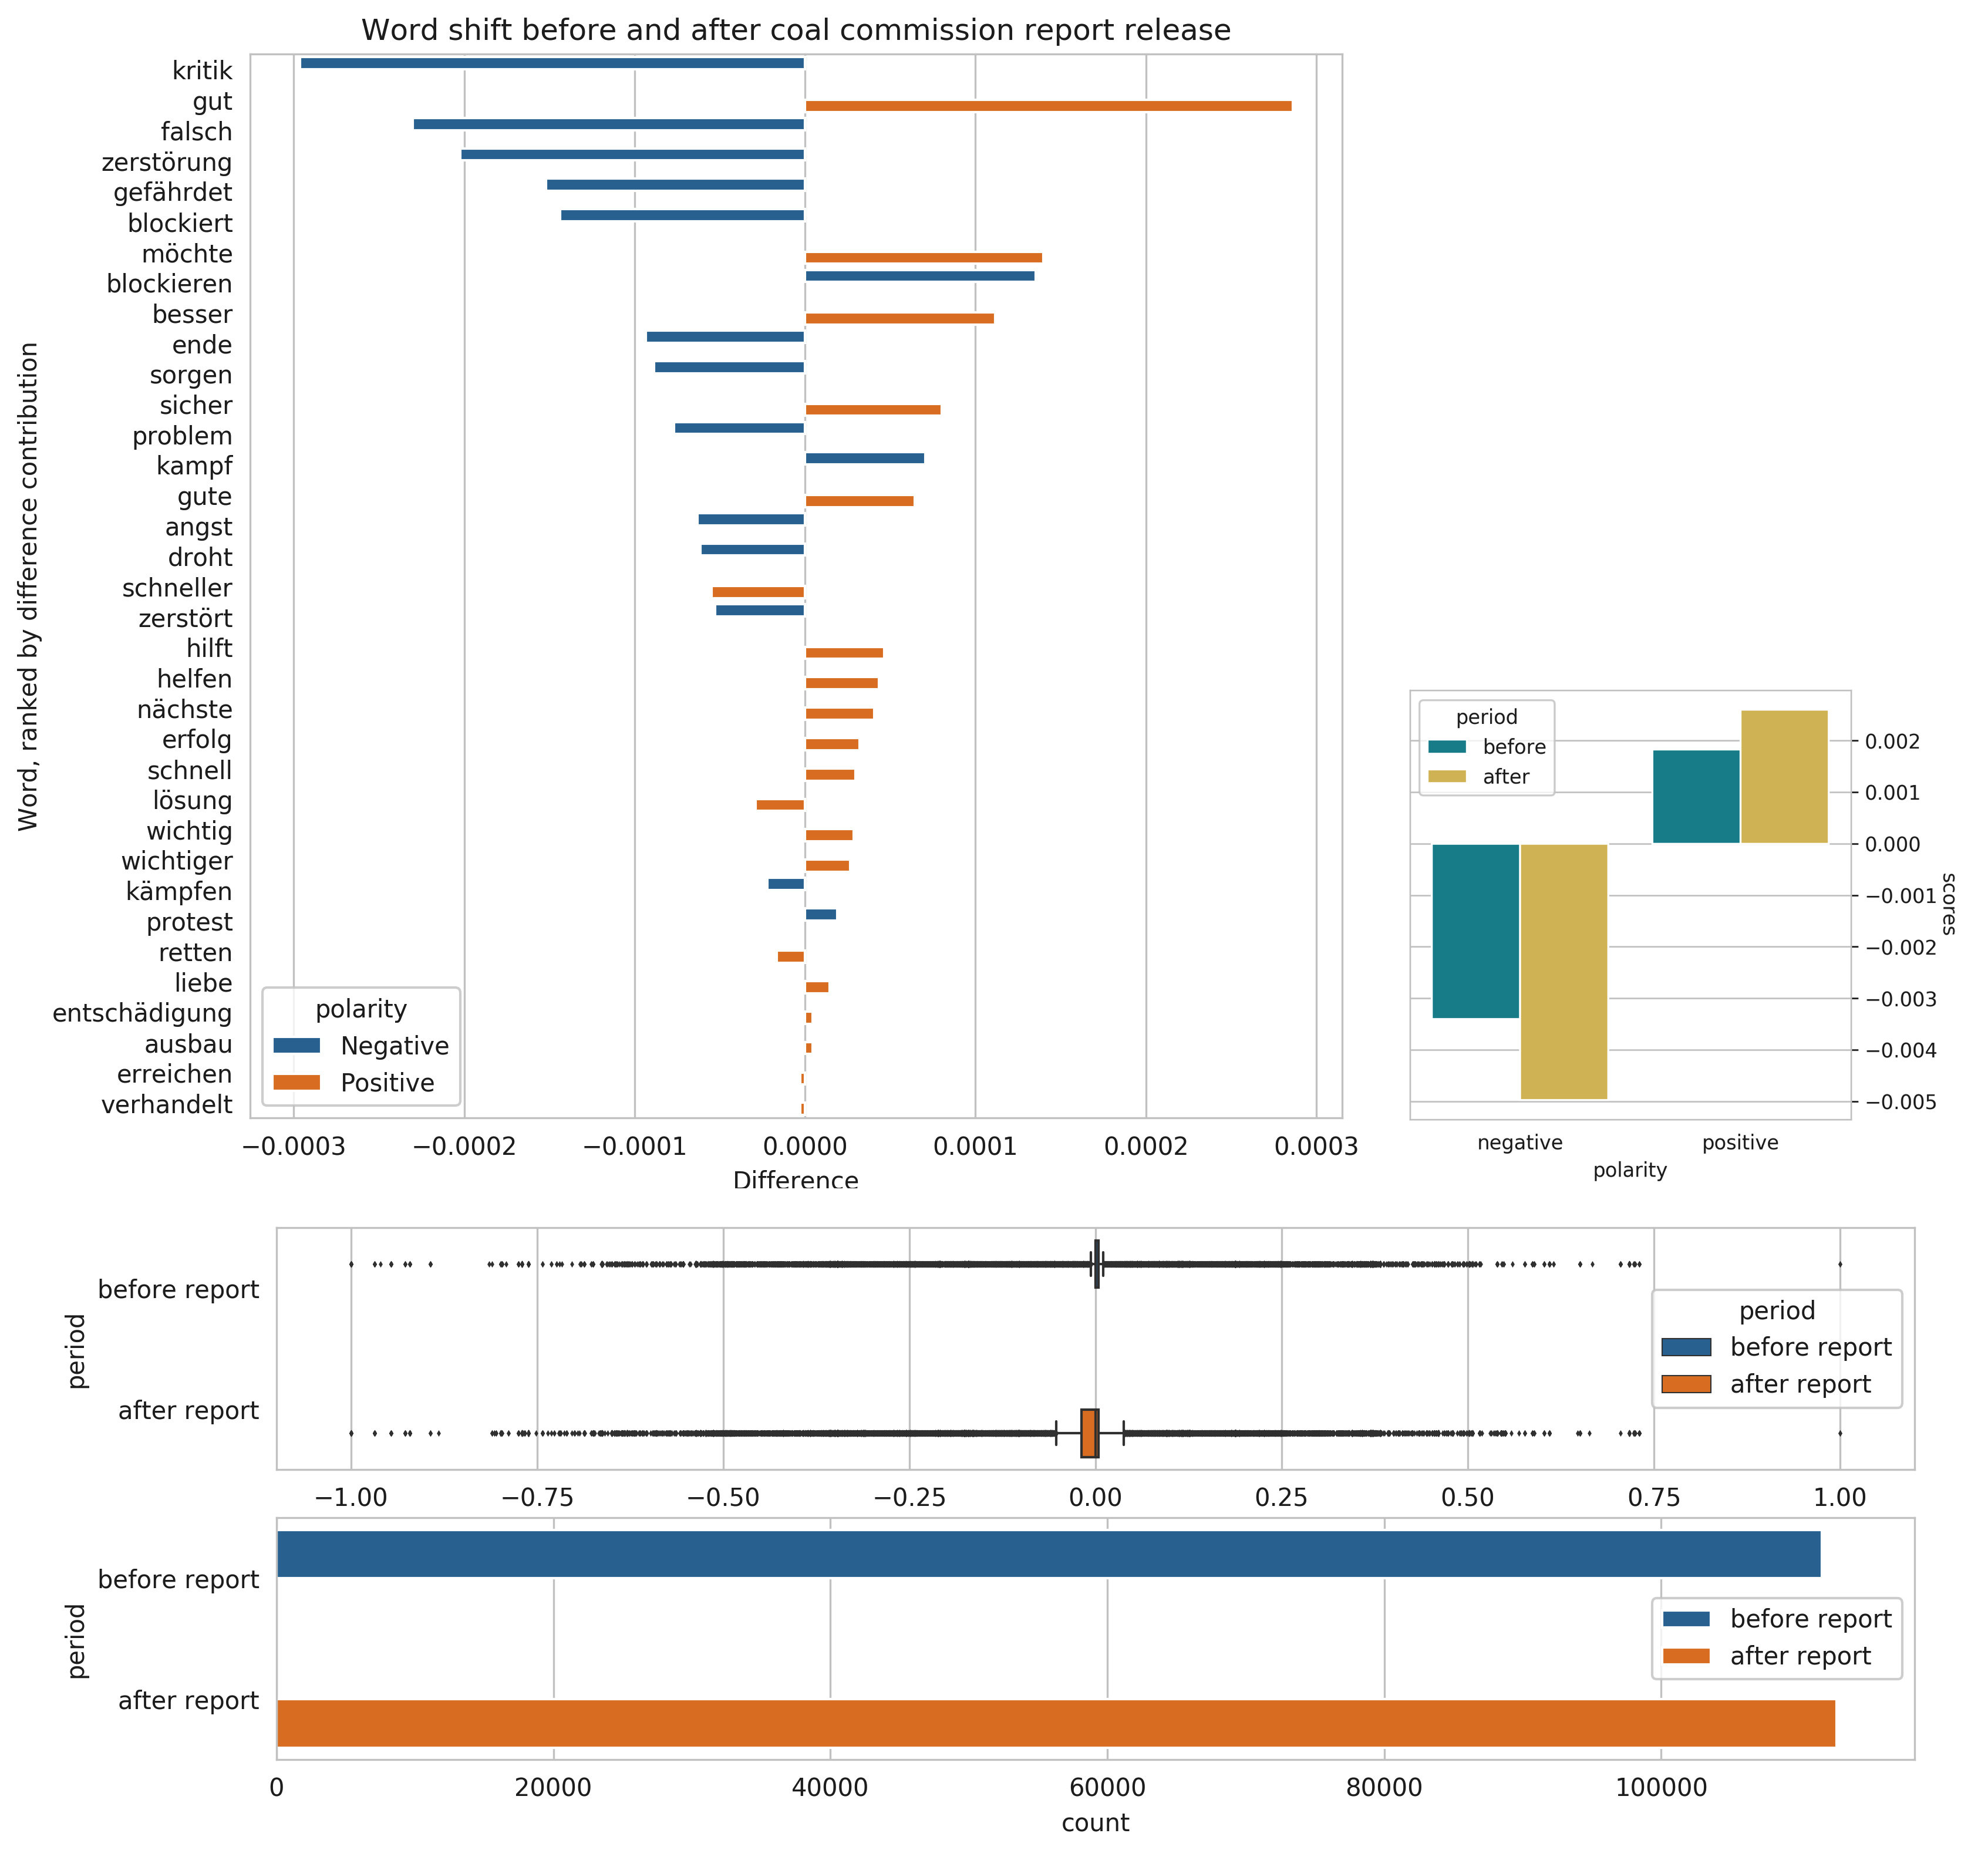
\includegraphics[width=\linewidth]{figures/wordshift_coalcomm_report_composite}
	\end{center}
 	\caption{\textbf{Word shift graph comparing tweets made before and after the release of the report of the coal commission.} The reference text is roughly 112000 tweets from the coal dataset from 1 January 2017 to 25 January 2019. The comparison texts is roughly 113000 tweets from the coal dataset from 26 January 2019 to 29 February 2020. An orange bar indicates a word with a positive polarity score. A blue bar indicates a word with a negative polarity score. Words on the right side are contributing to an increase in positive sentiment after the release of the coal commission report. Words on the left side are contributing to an increase in negative sentiment after the release of the coal commission report. Words with a blue bar on the left side of the graph and words with an orange bar on the right side of the graph are more prevalent in the tweets before the release of the coal commission's report. Words with a blue bar on the right side of the graph and words with an orange bar on the left side of the graph are more prevalent in tweets after the release of the coal commission's report. The subplot on the right shows the split in total word scores before and after the release of the coal commission report, sorted by word polarity.\protect\footnotemark}
	\label{fig:wordshift_coalcomm_report}
\end{figure*}
\footnotetext{Translation: good, criticism, wrong, destruction, endangered, wants, blocked, criticized, better, end, block, worry, safe, problem, fight, good, fear, destroyed, threatened, helps, important, next, help, fast, faster, more important, success, protest, fight, solution, love, save, compensation, expansion, solidarity}

Looking at Fig. \ref{fig:wordshift_coalcomm_report}, the first observation is that there are some very similar words on the list, for example ``gut''/``gute''\footnote{Translation: good} and ``zerstörung''/``zerstört''\footnote{Translation: destruction}, which are essentially different forms of the same word. This is a feature of the German language, and will be discussed in a later section.

% discuss word shift balances
In Fig. \ref{fig:wordshift_coalcomm_report}, the words are labelled by colour according to their individual polarity. In Fig. \ref{fig:wordshift_coalcomm_report}, we can see that the usage of both negative words as well as positive words is more common in the tweets made before the release of the coal commission's report. This suggests that there was a fiercer debate on coal during the period of the coal commission, as opposed to after, when it released its final results.

The split in the balance of scores arising from positive and negative words, before and after the release of the coal commission's report, however, suggest that there is an increase in polarisation of sentiments on Twitter after the coal commission process. This helps to explain why, looking at the sentiment score on 26 January 2020, there does not appear to be a significant difference in the score compared to the periods immediately before and after.

% word shift climate
In addition, in order to understand the debate on the German coal exit on Twitter, it is necessary to compare it to other debates on Twitter. Here, the climate debate is used as a reference. Fig. \ref{fig:wordshift_coal_climate} shows the word shift graph comparing the coal tweets against the climate tweets. In terms of the words that are driving the differences between the two datasets, the trends are largely similar to that in the previous figure comparing the tweets before and after the release of the coal commission's report. This means that positive and negative words both tend to appear more often in the climate dataset compared to coal.

In addition, the split in the balance of scores arising from positive and negative words between coal and climate tweets suggest that overall, sentiments in coal tweets are less polarised compared to that of climate tweets. This is not immediately apparent from the sentiment score timeseries plots, as those show the daily average sentiment score. This suggests that there might be more consensus on the coal debate on Twitter as compared to climate, which is not a surprising result as the coal debate can be considered as a sub-debate within the climate debate, which encompasses other topics.

\begin{figure*}
	\begin{center}
		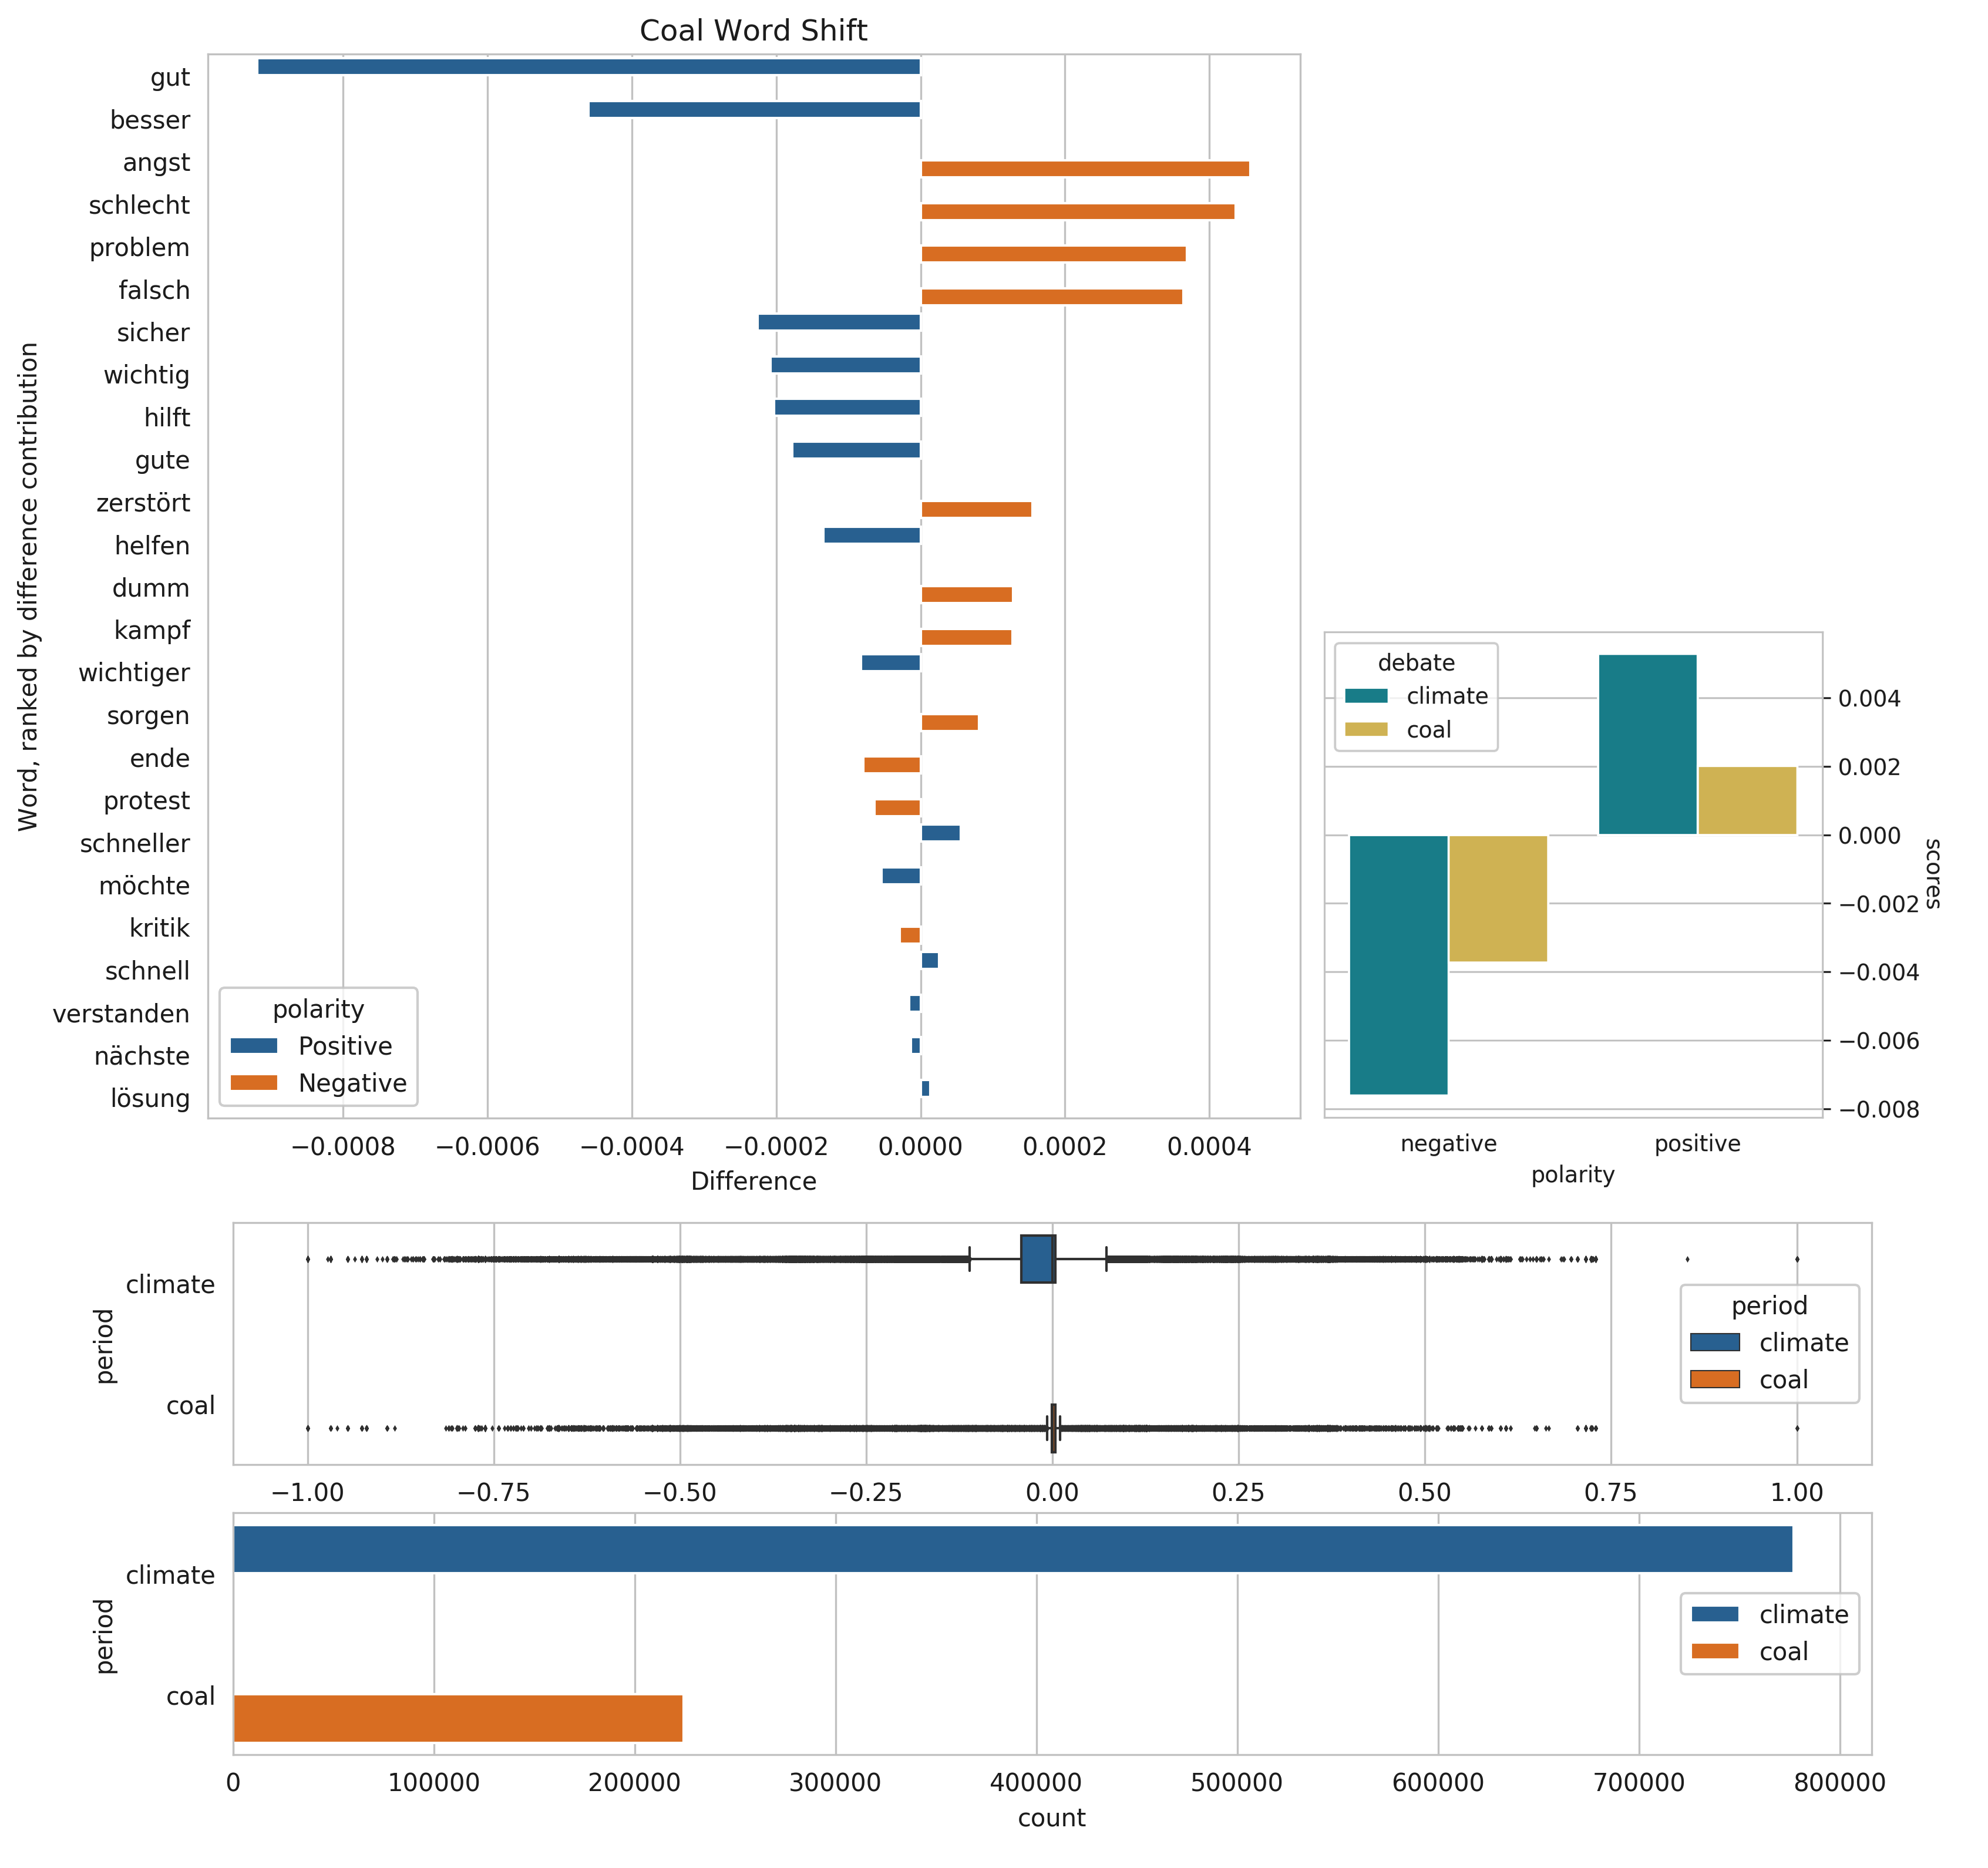
\includegraphics[width=\linewidth]{figures/wordshift_coal_climate_composite}
	\end{center}
	\caption{\textbf{Word shift graph comparing coal tweets to climate tweets.} The reference text is roughly 777000 tweets from the climate dataset from 1 January 2017 to 29 February 2020. The comparison texts is roughly 224000 tweets from the coal dataset from 1 January 2017 to 29 February 2020.}
	\label{fig:wordshift_coal_climate}
\end{figure*}


\subsection*{Network Analysis.}
% [T: 750, C: 800]
% should some of this go to Method instead?
\begin{figure*}
	\begin{center}
		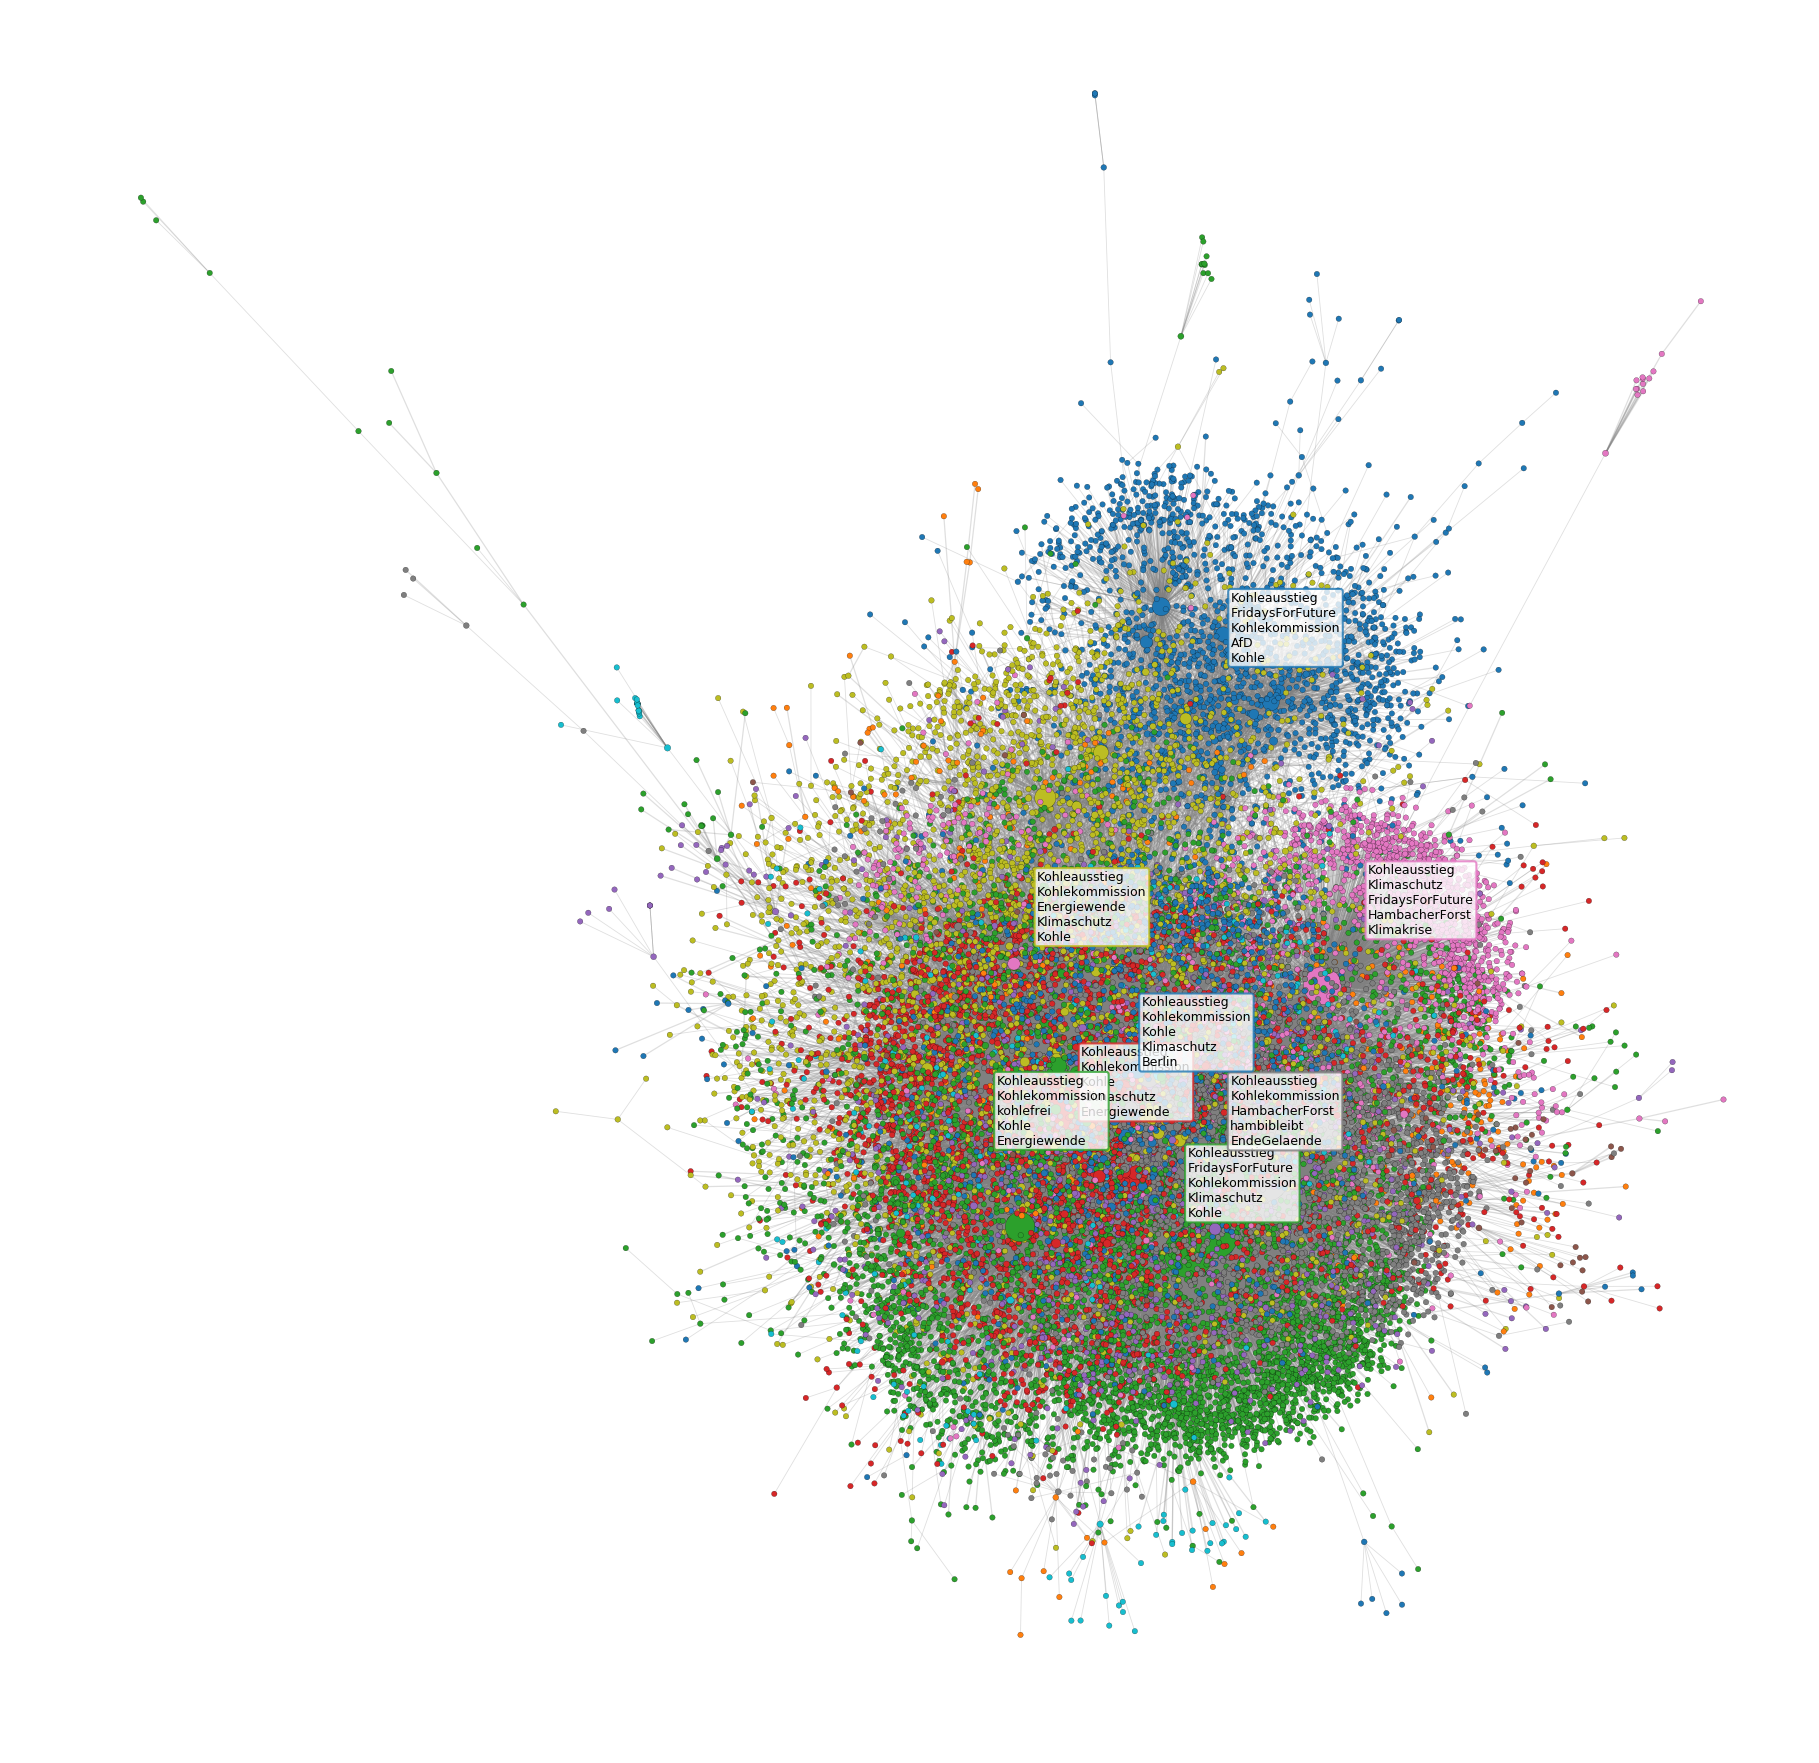
\includegraphics[width=0.8\linewidth]{figures/rt_network_ht2}
	\end{center}
	\caption{\textbf{Retweet network of the coal debate on Twitter.} The nodes represent Twitter users, and the edges between nodes represent the retweet relations. The node size is proportional to the total number of times the user has been retweeted by other members. The node colours correspond to the community that the community detection algorithm has identified it to be part of.}
	\label{fig:rt_network}
\end{figure*}

Another way of analysing the evolution of the coal debate on Twitter is to look at the retweet network of the dataset. In Twitter, a retweet refers to a re-post of a tweet, where another user chooses to share another user's tweet on their personal timeline. By taking Twitter users as nodes and retweets as edges, we can construct a retweet network and see which users retweet the most often from other users. From this, the community structure of the network can also be determined.

The community structure of a network refers to the appearance of densely connected groups of vertices, with only sparser connections between groups \citep{Newman8577}. The goal of most community detection algorithms, implicit or explicit, is to find the best trade-off between a large intra-cluster density and a small inter-cluster density. The strength of a community structure can be measured by its modularity, which is a measure of the extent to which like is connected to like in a network. It takes a value that is strictly less than 1, and it is positive if there are more edges between vertices of the same type than would be expected by chance, and negative if there are less \citep{Newman8577}. Modularity is defined as:

\begin{equation}
\label{eq:modularity}
Q = \frac{1}{2m} \sum_{i,j} \left(A_{ij} - \frac{k_i k_j} {2m}\right) \delta (c_i c_j)
\end{equation}

where $m$ is the total number of edges in the network, $A_{ij}$ are the elements of the adjacency matrix, or the number of edges between vertices $i$ and $j$, $c_i$ is the label of the community to which the node i is assigned, and $k_i$ is the degree of node i.

Community detection algorithms perform maximisation of modularity, and from the definition of modularity above, a good partitioning of a network is therefore one in which there are fewer than expected edges between the communities.

In this study, the fast-greedy community detection algorithm is used \citep{Clauset2004}. It is a popular algorithm for large networks due to its low computational cost and operates via hierarchical agglomeration.

\begin{figure*}
	\begin{center}
		\includegraphics[width=\linewidth]{figures/rt_network_ht_period4_edited2}
	\end{center}
	\caption{\textbf{Retweet network for period before release of coal commission report.} The top 5 hashtags within each community show that the debate is fairly homogenous, with little variation in the hashtags. The network also shows that there community partition is not particularly strong, with different communities clustered close to each other with retweets between communities.}
	\label{fig:rt_network_bef}
\end{figure*}

\begin{figure*}
	\begin{center}
		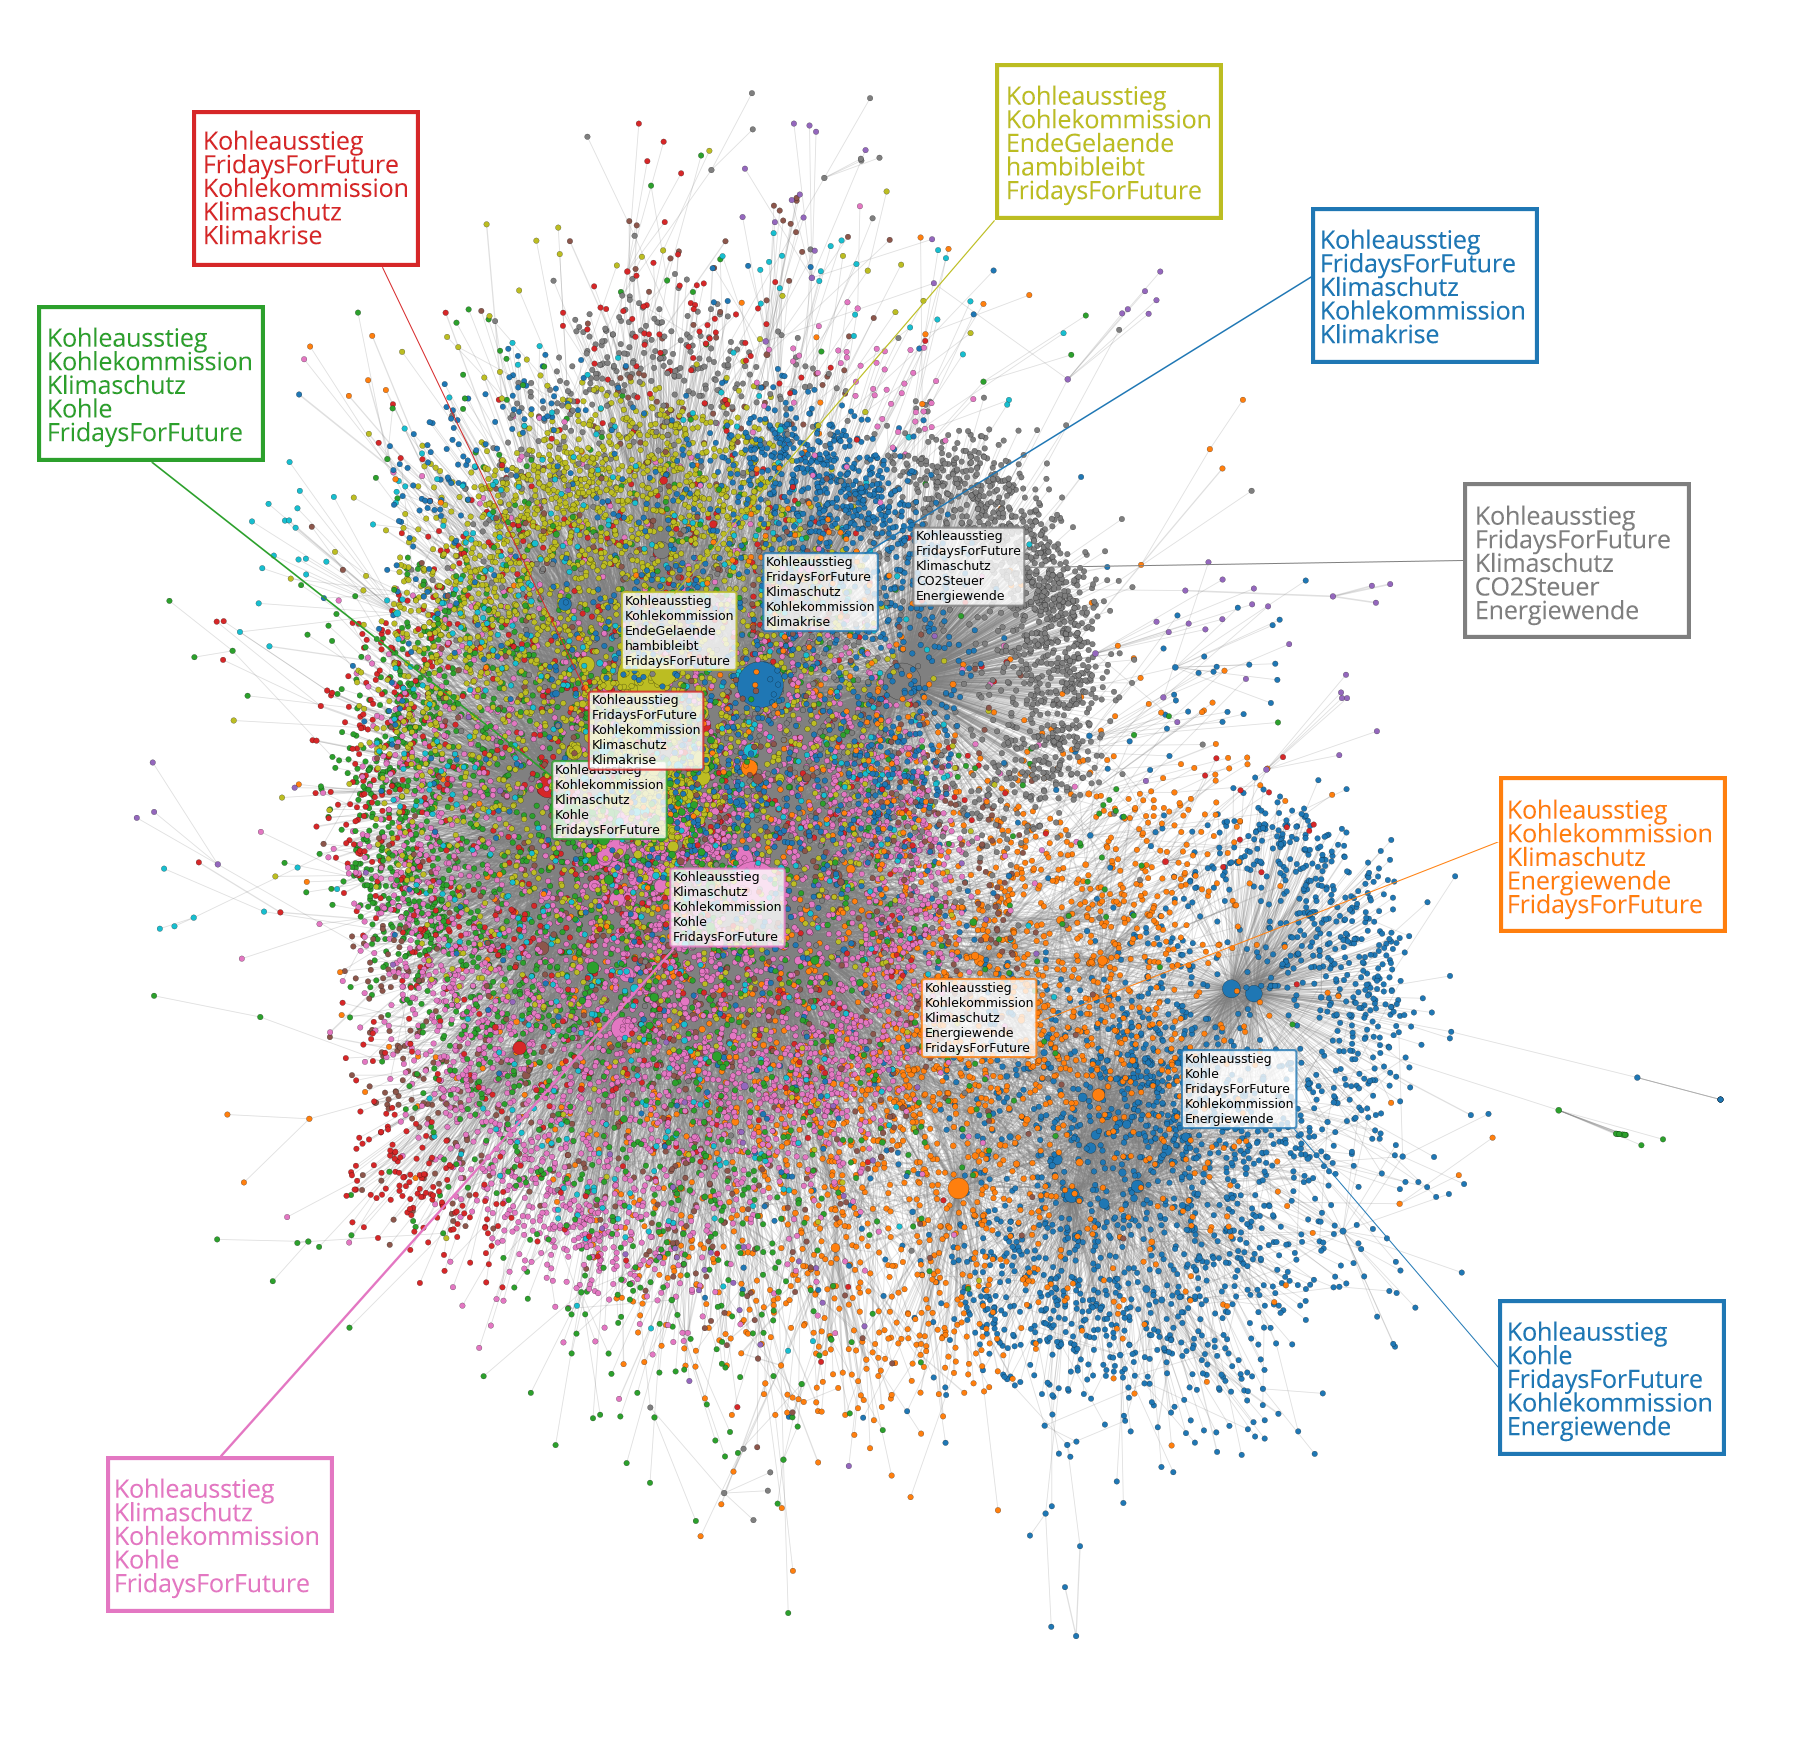
\includegraphics[width=\linewidth]{figures/rt_network_ht_period3_v3}
	\end{center}
	\caption{\textbf{Retweet network for period after release of coal commission report.} The top 5 hashtags within each community show that the debate remains fairly homogenous, similar to the network before the release of the commission's report, with little variation in the hashtags. However, there is an emergence of several sub-debates in this network, with unique hashtags like ``EndeGelaende'' and ``CO2Steuer'', showing that there is some evolution in the coal debate on Twitter.}
	\label{fig:rt_network_aft}
\end{figure*}

Fig. \ref{fig:rt_network_bef} and \ref{fig:rt_network_aft} show the two retweet networks of the period before and after the release of the coal commission's report respectively. Within each network, for communities with 500 nodes or more, the top 5 hashtags that are used in the community are also displayed. Looking at Table \ref{table:rt_network_mod}, the modularity scores are not significantly different from each other before and after the release of the coal commission report. This suggests that there has not been much change in the community structure of the retweet networks. However, looking at the number of nodes before and after suggests that there were more users involved in the coal debate on Twitter after the process of the coal commission. This suggests that over the course of the coal commission, there was discussion generated as a result of the process and events of the commission. This discussion was not just a result of an increase in the number of tweets by existing Twitter users in the coal debate, but also resulted from an increase in users. As the modularity score does not change, this suggests that the increase in users in the coal debate could have come from users within their own communities involving other users in their network who were previously not involved in the coal debate to join the coal debate.

Furthermore, the top 5 hashtags in the largest communities in the tweets made before and after the release of the coal commission report reveal that the main topics of discussion do not change much. The top 2 hashtags that appear in both periods are ``Kohleausstieg'' and ``Kohlekommission''\footnote{Translation: Coal exit, Coal commission}, and the other common hashtags in the two period include ``FridaysForFuture'', ``Klimaschutz'', ``Kohle'', ``HambacherForst'', ``Klimakrise'', and ``Energiewende''\footnote{Translation: Fridays for Future, Climate policy, Coal, Hambach Forest, Climate crisis, and Energy revolution}. However, the emergence of some sub-debates can be seen in Fig. \ref{fig:rt_network_aft}, with the appearance of a two communities -- one contianing the hashtag ``CO2Steuer''\footnote{Translation: CO2 tax} and another containing the hashtag ``EndeGelaende''\footnote{Translation: End of the land}, which refers to an environmental activist organisation which strongly protests the continuation of coal mining and coal-fired power production in Germany. 

One limitation of the fast-greedy algorithm used here is that it tends to form quickly large communities at the expenses of small ones \citep{Fortunato2010}. There are other community detection algorithms that can be used, but others are often much more computationally expensive due to the increase in complexity. In addition, studies show that the modularity score of large-scale social networks is typically greater than 0.5 \citep{Blondel2008}. This suggests that the community structure of the retweet network of the German coal debate on Twitter is not particularly strong, which is reflected by the homogeneity seen in the networks in Fig. \ref{fig:rt_network_bef} and \ref{fig:rt_network_aft}, with different communities clustered close to each other and many retweets between the communities. 

\begin{table}[htbp]
\begin{center}
	\caption{Size and modularity scores of coal retweet networks for the entire period, before the release of the coal commission's report and after the release of the coal commission's report}
	\label{table:rt_network_mod}
	\begin{tabular}{| l | p{2.5cm} | p{2.5cm} | l |}
		\hline
		Period & Before release of coal commission report & After release of coal commission report & Overall \\ \hline
		Nodes & 8926 & 19348 & 24267 \\ \hline
		Edges & 21312 & 48565 & 67093 \\ \hline
		Modularity score & 0.500 & 0.497 & 0.470 \\ \hline
	\end{tabular}
\end{center}
\end{table}


\section{Discussion} \label{sec:discussion}
\subsection*{Limitations.}
\subsubsection*{Sentiment Analysis}
% caveats of using dictionary methods for sentiment analysis
% [T: 500, C: 430]
The primary method of text analysis in this work has been sentiment analysis. As detailed earlier in the section on related work, there are two type of methods for sentiment analysis: lexical-based and machine-learning-based. Lexical, or dictionary-based methods make use of a predefined list of words, where each word has an associated sentiment or polarity weight. The results of lexical-based methods are thus heavily reliant on the dictionary used, and the context in which they were created \citep{Goncalves2013}. In this study, a pre-made, publicly available German dictionary, SentiWS, was used. It is a general resource, and not uniquely created for the context of studying the coal debate on Twitter. As a result, the words available in the dictionary may not reflect the full spectrum of words used in the coal debate, nor does it account for slang, which is common on social media networks but is rarely supported in dictionaries \citep{Hu2013}.

Some of the limitations of using dictionary methods are also evident from the results presented. In the cases where positive spikes were detected, further analysis of the tweet driving those spikes revealed that the intended sentiment of the text was not in fact positive, but rather sarcastic. Language construction is nuanced, and by reducing words to singular scores, some meaning will inevitably be lost. This will lead to a simplified result, which requires further analysis, as in the case here, to reveal the original sentiment.

One way of addressing this issue would be to use the alternative method, which is to use machine learning methods. Such methods often rely on supervised classification approaches, where sentiment detection is framed as a binary (i.e. positive or negative). Supervised approaches by nature require labelled data to train classifiers \citep{Pang2002}. This is advantageous in one sense as it allows for flexibility in creating trained models for specific purposes and contexts, but also has its drawbacks in that labelled data may not always be available. This means that existing labelled data may not always be suited for new data, as in the case of applying training data from standard long-form text to analyse social media text. Moreover, manually labelling data and creating a new data set is time intensive and costly.

No one method of sentiment analysis can replicate something that is fully manually classified, but its benefits, especially with dictionary methods, come in the form of its ease of automation, as well as speed in producing results. It is important, however, to take into account the limitations of such a method when analysing the results, as is in the cases presented above.

\subsubsection*{The German Language}
% limitations of language analysis in German
% [T: 300, C: 300]
Majority of the work done on sentiment analysis is conducted on the English language. In this study, the analysis is done on tweets in German as the policy case study is in Germany. There is one drawback of analysing German text with a dictionary-based approach of sentiment analysis -- compound words are a significant feature of the language, while dictionary methods typically only contain the root words. As a result, the method used here in this study will not pick up compound words. This is because the method of splitting sentences into words here is to identify the spaces in the words. Compound words will thus not be identified as they will not match either of the root words when the words in the sentences are matched to entries in the SentiWS dictionary.

Another feature of the German language is the use of declension. German declension is the paradigm used by the language to define all the ways articles, adjectives and sometimes nouns can change their form to reflect their role in the sentence: subject, object, etc. The ending of words can therefore take different forms, depending on the language case or grammatical gender in use. Within SentiWS, this is accounted for -- Fig. \ref{fig:sentiws_example} shows that for each root word, there are also its inflections in the same entry. Therefore, when a word is identified in the sentiment analysis process, so will all of its inflections, and all word forms will have the same polarity score. However, in the supporting analysis of word shifts, a simple frequency method is used to identify the top words driving the differences between texts, hence all the word forms are distinguishable. This can be seen in Fig. \ref{fig:wordshift_coalcomm_report} and Fig. \ref{fig:wordshift_coal_climate} where multiple word forms of the same root word appear.

\subsubsection*{Social Media data}
% drawbacks of using social media data, how to handle
% [T: 700, C: 700]
In addition to the limitations of a lexicon-based sentiment analysis method as well as the difficulties in analysing the German language, the biggest consideration when evaluating this study is the source of the data: Twitter. Twitter is a form of social media, and while using social media data offers many benefits as an alternative to conventional surveys in measuring public opinion, it also has several limitations as well.

Firstly, the assumption that Twitter posts represent an honest expression of public opinion may not necessarily hold true. The public nature of social media could induce a stronger social desirability bias than in the context of traditional survey responses, but the extent to which this occurs is unknown \citep{Klasnja2018}.

% representativeness
In comparison to traditional surveys, one crucial advantage that is lost with social media is the opportunity to control the sampling frame. Traditional surveys attempt to guarantee a known probability of any individual in the population being asked a survey question. With social media, however, the sampling is random, and thus it is not known the likelihood that someone has been asked a ``question'', nor the likelihood of a response \citep{Klasnja2018}. In analysing public opinion on social media, researchers do not ask the ``respondents'' a question, but rather depend on participants to reveal their opinion. This may raise an issue with the representativeness of the responses, as the set of people offering unprompted opinions on a topic may be more passionate or different in many ways from the set of people who offer opinions on that topic when explicitly asked. There is thus a big missing data problem when trying to analyse public opinion on Twitter, and results from Twitter cannot be generalised directly from Twitter responses to standard survey populations of interest.

Furthermore, Twitter users are not representative of national populations, something that is well documented \citep{Duggan2015, Mislove2011, Malik2015}. In the United States, it has been found that the most populous counties are overrepresented \citep{Mislove2011}, and there are also significant biases towards younger users and users of higher income when comparing geotagged tweets and census data \citep{Malik2015}. Evaluating the representativeness of Twitter users in Germany, however, is not straightforward, as Twitter does not record precise demographic information. Analysis of the geographic representation of users in Germany contributing to policy topics on Twitter reveal that there is a higher concentration of users in constituencies of high population density such as Berlin, Hamburg, Munich, and Cologne \citep{Fernandez2014}, but it is unclear whether these figures are representative of the national population. As such, in this study, there has not been an attempt to generalise the results about the coal debate on Twitter to the national coal debate, as there is not enough information about the user demographics on Twitter to be able to make these generalisations.

% slang, emojis
Another aspect of analysing social media data is the language differences used on social media. Texts in social media are often short, and thus using a dictionary that is trained using general texts like SentiWS might not be appropriate as it does not have sufficient aggregated information to measure the overall sentiment of a post. Moreover, slang and colloquial language is often used on social media, comprising new expressions that may not be represented on standard dictionaries. The short, unstructured, fast-evolving, and domain-specific nature of posts on social media mean that it is difficult to apply general language analysis tools to social media posts \citep{Hu2013}.

In addition to the usage of slang on social media, the use of emoticons, or emojis is also prevalent on social media. Emoticons are primarily face-based and represent happy or sad feelings, although a wide range of non-facial variations exist: for instance, <3 represents a heart and expresses love or affection. In the simplest form of a dictionary-based method for sentiment analysis, emoticons are discarded when pre-processing the text, and thus could lead to the loss of valuable information when aggregating sentiment. One way to tackle this is to extract polarity from emoticons, and attach a polarity weight to each emoticon. This can then be used in combination with the dictionary method to get a better overall sentiment score for a tweet. However, issues remain as to how to scale the polarity of emoticons, which can be subjective across different users.

\subsection*{Policy Implications.}
% [T: 750, C: 830]
The findings presented above have several policy implications. Linking back to the original task set out in this study, this project aimed to identify whether there was an effect on public opinion on the German coal exit throughout the entire decision-making process of the coal commission. Based on the changes seen in the daily average sentiment scores of tweets about coal on Twitter, it can be concluded that there was indeed an effect.

% Increasingly negative sentiment
Furthermore, this effect was negative, as there was a clear negative trend of average sentiment scores throughout the entire period of study from 1 January 2017 to 29 February 2020. The negative trend of coal tweets is also not fully reflected in the daily averages, due to false positive spikes. Further analysis of the tweets that were driving large negative sentiments showed that this was due to the usage of negative words to i. express support for coal exit movements and ii. criticise the efforts and results of the coal commission.

These results show that within the online community on Twitter, discussion about the German coal exit and the coal commission was largely negative, and grew increasingly negative over time. While the online community on Twitter is not representative of the entire population of Germany, this result still clearly indicates that online discourses on coal are largely dominated by negative views on coal. This is likely to be due to the increase in calls for greater climate action as part of the Fridays For Future movement that gained traction over the course of 2019. This sends a clear signal to policy-makers that environmental policies will be scrutinised on online communities, and any policies that are made that may be perceived to not prioritise the environment strongly enough are likely to be unpopular. Whilst policy-making is not meant to be populist, it is nevertheless important for policy-makers to understand sentiments on the ground, and how policies will be received when introduced and enacted. This is particularly important for future planning, as many climate and environmental policies will only see the results of the enacted policy in the long term, when it comes to impacts such as reducing carbon emissions and mitigating climate change.

% No consensus?
Another possible implication for public policy making from the results of this study is that about consensus-forming. As discussed previously, the coal commission was a multi-stakeholder commission that was meant to bring together different stakeholders in the coal (and by extension energy and environment) sector in Germany in order to negotiate a best-case scenario for phasing out coal in Germany. While the commission eventually agreed on a final phase-out date, as well as the amount for structural funds to support those affected by the phase-out, this was seen as a compromise, and multiple criticisms of the commission's report have since been published. This is also reflected in the discourse on Twitter, suggested by both the variation in the daily average sentiment scores during the period surrounding the entire coal commission process, as well as the balance of sentiment scores which show an increase in both positive and negative words in the coal discourse on Twitter. This is also further supported by looking at the retweet networks of the coal debate before and after the conclusion of the coal commission with the release of its report, as the communities identified did not appear to become stronger or more unified, signifying a lack of consensus building.

This suggests that while efforts to bring together different stakeholders in the coal sector by using the coal commission as a form of public policy-making managed to produce a final result for the commission, this did not translate to the online community on Twitter. The possible policy implications for this are that while multi-stakeholder commissions may be useful in bringing together different stakeholders with different interests within a specific sector, results may not necessarily translate to the wider public, and hence such commissions cannot be seen as a means for building public consensus on a topic, nor can they claim to.

\subsubsection*{Further Work}
There remains many possible avenues for research on the coal debate on Twitter. As discussed in the section on limitations, there are many alternative methods that could be used, such as using machine-learning methods for sentiment analysis, or building a better, and more nuanced dictionary suitable for analysing the language used on social media. However, in order for such research to complement policy-making, it is important to increase the representativeness of the data used. One possible extension of the current work would be to look into the the diversity of the Twitter users in this dataset in order to better understand the bias in using social media data. This could be followed by re-weighting data to balance out the biases, using methods like multilevel regression and post-stratification, which has been used in party and ideological identification on Twitter \citep{Barbera2015}, or to augment Twitter data with demographic information from other sources \citep{Barbera2015a, Bode2016}.

\section{Conclusion} \label{sec:conclusion}
This study has provided a general exploration of the German tweets on coal debate, through analysis of the tweets' sentiments and retweet networks. The results show that there is a negative trend in the sentiment of tweets over time, which is also reflected in the broader German debate on climate. This increasingly negative sentiment is supported when looking into the specific tweets that are driving the large negative spikes in daily sentiment scores. Further analysis of the content of these tweets show that negative language is being used to express the severity of climate change, and the role that coal plays in it. The coal commission is also, by extension, painted in a negative light. Furthermore, tweets that drive large positive spikes in the sentiment scores are also critical about coal and the role of the coal commission, suggesting that the negative sentiment is more pronounced than what is presented. Despite the increase in negative sentiments on Twitter, however, analysis of the retweet networks reveal that the community structure of the coal tweets do not change significantly, and hence there was not much interaction between different communities on the coal debate on Twitter. This reveals that despite the original intentions of the coal commission to bring together different stakeholders in the coal sector to come to a common result for the coal phase-out in Germany, this aim of consensus-building did not extend to the public on Twitter.

While the coal commission and the coal exit was well-covered in traditional media, this study provides an overview on the coal debate throughout the coal commission process on the social media site Twitter. Through social media, the general public can learn about current events surrounding the coal commission and the coal exit in Germany, and display their own opinions about the issues as well. Twitter may be a useful resource in understanding public opinion, as well as an unsolicited public opinion tool for policy makers.

%%% END TEXT %%%

\vfill
\rule{0.33\linewidth}{0pt}\\[-3.7ex] \rule{0.33\linewidth}{0.6pt}
\acknow{I would like to thank Prof. Slava Jankin and Prof. Dr. Jan Minx from the Mercator Research Institute on Global Commons and Climate Change (MCC) for co-supervising this thesis, and for their invaluable input. I would also like to thank Finn Müller-Hansen and Max Callaghan from MCC for their input in the development of the research design, and for their help with data collection. Thanks to MCC for the computational resources provided as well.}

\showacknow{} % Display the acknowledgments section
\clearpage
\section*{References}
% Bibliography

\bibliography{bibliography}
\clearpage

\appendix
\section{Appendix}

\clearpage
\section{Statement of Authorship}
I hereby confirm and certify that this master thesis is my own work. All ideas and language of others are acknowledged in the text. All references and verbatim extracts are properly quoted and all other sources of information are specifically and clearly designated. 

\subsection*{Date:} \today


\subsection*{Name:} Yuan Ting Lee


\subsection*{Signature:}

\end{document}
